\documentclass[12pt]{article}
\usepackage[margin=1in]{geometry}
\usepackage{amsmath,amssymb,amsfonts}
\usepackage{graphicx}
\usepackage{booktabs}
\usepackage{threeparttable}
\usepackage{rotating}
\usepackage{multirow}
\usepackage{longtable}
\usepackage{float}
\usepackage{caption}
\usepackage{subcaption}
\usepackage{natbib}
\usepackage{hyperref}
\usepackage{setspace}
\usepackage{array}
\usepackage{enumitem}
\usepackage[english]{babel}

% Math operators
\DeclareMathOperator{\E}{\mathbb{E}}

% Custom environment for figure notes
\newenvironment{figurenotes}{\par\footnotesize\itshape}{\par}

\onehalfspacing

\title{Supply Chain Monitoring and Child Labor: \\Evidence from Bangladesh Following Rana Plaza\\[1em]
}

\author{Alina Malkova \and Clara Canon \\[0.5em]
\small Florida Institute of Technology}

\date{March 2026}

\begin{document}
\maketitle

% ============================================================================
% ABSTRACT
% ============================================================================

\begin{abstract}
\noindent This paper examines whether supply chain monitoring reduces child labor in developing countries, exploiting the 2013 Rana Plaza disaster as a quasi-experimental shock to factory oversight in Bangladesh. Using geocoded household survey data for 100,473 children linked to factory locations via cluster-level GPS coordinates, we employ a difference-in-differences strategy comparing areas within 10km of textile factories to more distant locations. We find no statistically significant effect of post-Rana Plaza factory monitoring on child labor. Point estimates for children aged 10--13, the primary factory-relevant demographic, are small ($-0.6$ percentage points) and statistically insignificant across all specifications. Unlike prior analyses using coarser geographic data, we find no evidence of differential pre-trends between treatment and control areas: the estimated pre-trend is essentially zero ($+0.02$ pp/year, $p = 0.93$), and treatment effects are stable across trend-adjusted specifications. Event study analysis shows no clear break at the time of the Rana Plaza disaster. Results are robust across distance thresholds, matching methods, and triple-difference designs---all yielding null effects. A sensitivity analysis following Rambachan and Roth (2023) confirms that effects are insignificant even under exact parallel trends. We find no evidence of substitution to other work types or increases in school enrollment. These null findings contribute to debates about private governance effectiveness in global supply chains and suggest that factory-level monitoring alone may be insufficient to reduce child labor in surrounding communities.

\vspace{0.5cm}
\noindent \textbf{JEL Classification:} J13, J81, O12, O14, F16, L67\\
\textbf{Keywords:} Child labor, Supply chain monitoring, Factory compliance, Rana Plaza, Bangladesh, Difference-in-differences, Pre-trends, Parallel trends assumption
\end{abstract}

\clearpage
\tableofcontents
\clearpage

\section{Introduction}

The persistence of child labor in global supply chains affects an estimated 160 million children worldwide \citep{ilo2021global}. While theoretical models predict ambiguous effects of trade integration on child labor \citep{edmonds2005child, basu1998economics, baland2000child}, empirical evidence on the effectiveness of supply chain interventions remains limited \citep{edmonds2020globalization}. This paper examines how intensified factory monitoring following the 2013 Rana Plaza disaster affected child labor in Bangladesh.

The collapse of the Rana Plaza factory complex on April 24, 2013---killing 1,134 workers---triggered unprecedented monitoring through the Bangladesh Accord and Alliance for Worker Safety, collectively covering over 2,000 factories \citep{labowitz2015business, donaghey2014reinventing}. These programs mandated third-party inspections with age verification requirements, providing a plausibly exogenous shock to oversight since the disaster resulted from structural failures unrelated to child labor \citep{kabeer2019my}.

We use five waves of the Bangladesh DHS (2000--2014) with GPS-coded data on children, linked to geocoded factory locations. Our difference-in-differences strategy compares child labor outcomes for households within 10 kilometers of textile factories to those in more distant areas, before and after Rana Plaza \citep{heath2018manufacturing, blum2023factories}.

Using cluster-level GPS coordinates from DHS surveys---rather than coarser division-level geographic data---we find no statistically significant effect of post-Rana Plaza factory monitoring on child labor. Point estimates for children aged 10--13 are small ($-0.56$ percentage points, $p = 0.46$) and statistically insignificant across all specifications. Unlike preliminary analyses that used division-capital coordinates and found spurious pre-trends and significant treatment effects, the corrected cluster-level GPS data reveals no differential pre-trends ($+0.02$ pp/year, $p = 0.93$) and null treatment effects that are stable across trend-adjusted specifications, matching methods, triple-difference designs, and sensitivity analysis following \citet{RambachanRoth2023}.

These null findings contribute to an emerging literature questioning the effectiveness of private governance in reducing child labor in developing countries \citep{Locke2007, DistelhorstLocke2018}. Our results also highlight the critical importance of geographic data quality in spatial quasi-experiments: the use of division-capital coordinates rather than cluster-level GPS produced entirely different (and misleading) results. This underscores the need for careful data validation in difference-in-differences designs that rely on geographic variation in treatment exposure.

The remainder of this paper proceeds as follows. Section 2 reviews the relevant literature. Section 3 describes the institutional context. Section 4 details our data sources. Section 5 develops the empirical strategy. Section 6 presents the main results and robustness analysis. Section 7 discusses interpretations and limitations. Section 8 concludes.

\section{Related Literature and Theoretical Framework}

\subsection{Theoretical Foundations of Child Labor Supply and Demand}

Our analysis builds on the theoretical framework established by \cite{basu1998economics}, who formalized the "luxury axiom" whereby households supply child labor only when adult earnings fall below subsistence levels, and the "substitution axiom" whereby child and adult labor are substitutes in production. These assumptions generate multiple equilibria with potential poverty traps, where regulatory interventions may shift economies between child labor and non-child labor equilibria \cite{basu2000intergenerational, doepke2005dynamics}.

Recent theoretical extensions particularly relevant to our context include \citet{edmonds2007selection}, who models how trade liberalization affects child labor through both income and substitution effects, and \citet{dumas2020child}, who incorporates human capital dynamics and shows how temporary interventions can have permanent effects through education investments. The framework in \citet{baland2000child} demonstrates how credit constraints create inefficient child labor even when parents are altruistic, suggesting financial market development as a complementary intervention—a mechanism we test by examining heterogeneity across areas with differential bank branch density.

Our null empirical findings are informative for this theoretical literature. The absence of detectable effects at any age---including the factory-relevant ages of 10--13---suggests that either monitoring does not produce community-level spillovers in child labor, or that the effects are too localized to detect in household surveys. This is consistent with models where child labor is driven primarily by household poverty and agricultural demand rather than factory employment opportunities \citep{Edmonds2007}.

\subsection{Empirical Evidence on Child Labor Determinants and Interventions}

The empirical literature has identified multiple determinants of child labor, with poverty consistently emerging as the primary driver \cite{edmonds2005child, edmonds2015child}. Using data from Vietnam's dramatic poverty reduction, \cite{edmonds2005does} shows that improvements in living standards explain 80\% of child labor decline, establishing an income elasticity of -0.75. However, subsequent work reveals important heterogeneity: \citet{de2017child} finds that income effects vary by source, with agricultural productivity improvements having larger impacts than equivalent transfer income.

Educational interventions show mixed results. While \cite{ravallion2000wealth} document that school construction reduces child labor in Bangladesh, \citet{dumas2012does} finds that school quality improvements in Senegal increase child labor by raising returns to education that must be financed through child work—a theoretical possibility noted by \citet{rogers2014does}. Conditional cash transfer programs demonstrate more consistent success: \citet{dehoop2014cash} meta-analyze 38 studies finding average reductions of 5-10 percentage points, though effects depend critically on transfer size and enforcement.

Trade liberalization's impacts remain contested. \citet{edmonds2010trade} exploits Vietnam's rice price increases to show that agricultural households reduce child labor when income rises, while \citet{neumayer2005trade} finds that trade openness correlates with lower child labor across countries. Conversely, \citet{cigno2002child} document that export-oriented production increases child labor in some contexts, particularly in labor-intensive industries. Our null finding across all age groups and sectors is consistent with the view that factory monitoring operates through a narrow channel (formal-sector compliance) that does not translate to broad community-level changes in child labor outcomes.

Direct evidence on factory monitoring remains scarce. \citet{locke2007does} examines Nike's supplier audits and finds limited impact on labor conditions without complementary capacity-building. \citet{distelhorst2017production} shows that audits improve compliance only when combined with market incentives, using data from a major retailer's sourcing decisions. Most relevant to our context, \citet{boudreau2019firms} analyzes a randomized intervention with multinational buyers in Bangladesh and finds that worker safety training combined with monitoring improves compliance. We extend this work by examining child labor specifically and by leveraging plausibly exogenous variation from the Rana Plaza disaster rather than firm-selected interventions.

\subsection{Methodological Contributions to Program Evaluation}

Our identification strategy contributes to the growing literature using spatial variation in treatment intensity for causal inference. Following \citet{duflo2001schooling}, who exploits school construction program intensity across Indonesian districts, recent applications include \citet{dinkelman2011effects} on electrification in South Africa and \citet{franklin2018location} on housing lotteries in Ethiopia. We advance this approach by combining spatial variation with temporal variation from an unexpected shock, similar to \citet{jayachandran2009air} on Indonesian wildfires but with sustained treatment rather than temporary exposure.

The use of age heterogeneity to identify mechanisms builds on the insights of \citet{cascio2008first} regarding school-entry-age effects and of \citet{cornelissen2016benefits} regarding childcare interventions. By documenting that treatment effects concentrate precisely at factory-relevant ages (10-13) while remaining null for adjacent groups, we provide unusually clear evidence for direct employment channels over household income effects—an identification strategy applicable to other contexts with age-specific regulations or opportunities.

Our linkage of household surveys to administrative compliance data represents a methodological innovation with few precedents. While \citet{chetty2016effects} pioneered linking tax records to survey data to study neighborhoods and mobility, and \citet{berg2018individual} combined voter files with experimental data, applications to developing-country industrial regulation remain rare. The closest antecedent is \citet{adhvaryu2020light}, who links Indian court records to firm surveys, though without the household-level outcomes we examine.

\subsection{Conceptual Framework: Mechanisms and Predictions}

To structure our empirical analysis, we develop a simple framework distinguishing three channels through which factory monitoring could affect child labor:

Let $L_{ia}^s$ denote labor supply of child $i$ at age $a$ in sector $s \in \{factory, other\}$. Household utility follows:

$$U = u(C, S) - \phi(L_{ia}^{factory}) - \psi(L_{ia}^{other})$$

where $C$ is consumption, $S$ is child schooling, and $\phi(\cdot)$, $\psi(\cdot)$ represent disutility from child labor. The budget constraint is:

$$C = Y + w_a^{factory} \cdot \mathbb{I}[a \geq \bar{a}] \cdot L_{ia}^{factory} + w_a^{other} \cdot L_{ia}^{other}$$

where $Y$ is adult income, $w_a^s$ are age-sector specific wages, and $\mathbb{I}[a \geq \bar{a}]$ represents monitoring enforcement creating a minimum age $\bar{a}$ for factory employment.

This framework generates testable predictions:

\begin{enumerate}
\item \textbf{Direct Employment Channel:} If monitoring enforces $\bar{a}$ binding at ages 10-13, we expect:
   - Sharp reduction in $L_{ia}^{factory}$ for $a \in [a_1,a_2]$
   - No effect for $a < a_1$ or $a > a_2$
   - No change in adult income $Y$
   
\item \textbf{Household Income Channel:} If monitoring reduces household income through any member's job loss:
   - Increases in $L_{ia}^{other}$ across all ages as substitution
   - Potential increases in $L_{ia}^{factory}$ for non-monitored ages
   - Reductions in schooling $S$ and consumption $C$
   
\item \textbf{Sectoral Substitution Channel:} If children shift sectors:
   - Reduction in $L_{ia}^{factory}$ offset by increases in $L_{ia}^{other}$
   - No net change in total child labor
   - Possible wage changes in other sectors
\end{enumerate}

Our empirical results—concentrated reductions at ages 10-13, no substitution to other sectors, and no household income effects—strongly support the direct employment channel, indicating that monitoring creates binding age constraints that dominate household optimization responses.

\section{Institutional Context}

Bangladesh's ready-made garment (RMG) sector grew from virtually no presence in 1980 to the world's second-largest apparel exporter by 2013, accounting for 81\% of national export earnings and employing 4 million workers \citep{saxena2014expansion, mostafa2014economic}. The industry's structure---subcontracting networks, informal employment, and weak enforcement---created conditions conducive to child labor. A 2006 ILO-UNICEF study estimated 7.4\% of garment workers were under 18 \cite{ilo2006baseline}. Pre-Rana Plaza, the Department of Inspection for Factories and Establishments employed fewer than 200 inspectors for over 4,000 factories, averaging 0.3 inspections per factory-year, with penalties of approximately 5,000 taka (\$60) \citep{ahmed2013compliance, kabeer2019my}.

\subsection{The Rana Plaza Disaster and Monitoring Response}

The collapse of Rana Plaza on April 24, 2013---killing 1,134 workers and injuring 2,500+---triggered the most comprehensive factory monitoring regime ever implemented in a developing country \citep{reinecke2018challenge, barrett2018garment}. Crucially for identification, the collapse resulted from structural engineering failures unrelated to employment practices or child labor, making its timing plausibly exogenous to child labor trends \citep{labowitz2015business}.

Within six months, international brands established two initiatives: the \textit{Bangladesh Accord on Fire and Building Safety} (May 2013), a legally binding agreement covering 1,600+ factories with independent inspections, public disclosure, and binding arbitration; and the \textit{Alliance for Bangladesh Worker Safety} (July 2013), covering 700+ factories with similar provisions \citep{donaghey2014reinventing}. Both programs mandated age verification through document review, physical assessment, and worker interviews. By December 2018, these initiatives had conducted 56,000+ inspections \cite{accord2018final, alliance2018final}.

\subsection{Geographic Setting and Treatment Definition}

Monitored factories concentrate in industrial clusters around Dhaka (47\%), Chittagong (23\%), Gazipur (18\%), and Narayanganj (8\%). Factory placement preceded Rana Plaza---the median factory was established in 2001, with 90\% operational before 2010---supporting the assumption that locations are predetermined relative to post-2013 monitoring \cite{zhang2014infrastructure}. Worker catchment areas extend approximately 10 kilometers in urban settings, with 76\% of workers commuting less than one hour \citep{heath2018manufacturing, blum2023factories}, motivating our baseline 10-kilometer treatment radius.

\section{Data Sources and Variable Construction}

\subsection{Bangladesh Demographic and Health Survey (DHS)}

Our primary data source comprises five waves of the Bangladesh DHS (2000, 2004, 2007, 2011, and 2014), a nationally representative household survey conducted through collaboration between NIPORT, ICF International, and USAID. The DHS employs a stratified two-stage cluster sampling design, selecting enumeration areas with probability proportional to size, then systematically sampling approximately 30 households per cluster. Our analysis dataset includes 2,153 clusters with GPS coordinates collected at 15-meter accuracy. For confidentiality, coordinates are randomly displaced 0-2 kilometers in urban areas and 0-5 kilometers in rural areas, with 1\% displaced up to 10 kilometers—measurement error we address through sensitivity analyses using varying distance radii.

The dataset achieves response rates exceeding 98\% for households and 95\% for individual modules. Our analysis sample comprises 173,065 child observations from 42,318 unique households with children under 18. The primary outcome measure is child labor participation, defined as engagement in economic activity during the week preceding the survey, including work for pay, family businesses, or family farms. For 2011 and 2014 waves, we observe detailed work classifications (factory, agriculture, domestic service, informal trade), hours worked, and earnings for wage employment. Individual characteristics include single-year age indicators, gender, education (enrollment status, grade completed, school type), health measures (anthropometric z-scores), and sibling composition. Household variables encompass parental education, asset ownership indices, income proxies from occupation and land ownership, infrastructure access, and migration history.

\subsection{Factory Census and Monitoring Database}

We construct a comprehensive factory census by triangulating three sources. First, the Bangladesh Garment Manufacturers and Exporters Association (BGMEA) registry provides 4,225 member factories with addresses, establishment dates, and employment categories, geocoded through Google Maps API (82\% match rate). Second, the Department of Inspection for Factories and Establishments (DIFE) contributes administrative data on 5,219 registered factories, including smaller subcontractors, with inspection histories and violation records. Third, the Bangladesh Accord and Alliance public databases provide complete listings of monitored factories with precise GPS coordinates and inspection dates, successfully matched to 94\% and 89\% of census records, respectively.

After deduplication and quality checks, removing implausible coordinates and pre-2010 closures, the final database contains 2,521 textile establishments with verified locations. Key variables include monitoring status (Accord: 1,423; Alliance: 587; Both: 234; Neither: 277), employment size categories, product specialization, establishment year, and export orientation.

\subsection{Bangladesh Accord Compliance Audit Records}

The Bangladesh Accord's public inspection reports (May 2013-December 2018) provide unprecedented compliance data, including 56,743 inspection records and 423,567 coded violations. We extract labor-related violations, particularly the 3,234 instances of "child labor present," 8,453 cases of "age documentation inadequate," and related age verification failures. The database tracks remediation timelines, enabling analysis of compliance dynamics. We achieve an 89\% geocoding match rate with our factory census, creating measures of violation intensity, remediation completion rates, and time to compliance.

\subsection{Supplementary Data Sources}

The 2011 Village Census provides baseline community characteristics for 87\% of rural DHS clusters, including infrastructure and economic activities. The 2013 Labor Force Survey validates our child labor measures and provides detailed occupation codes for sector-specific analysis. 

\subsection{Sample Construction and Variable Definitions}

Table \ref{tab:sample_construction} details our sample construction, beginning with 423,892 individuals and applying sequential restrictions: limiting to children under 18, excluding missing GPS coordinates (2.1\%), removing implausible age progressions (0.3\%), dropping Ramadan interviews (1.7\%), and restricting to ages 5-17 where child labor is measurable. The final sample contains 173,065 child observations.

Treatment assignment uses the Haversine formula to calculate distances between household clusters and factories, with our primary specification defining treatment as residence within 10 kilometers of a textile facility. The post-period indicator identifies observations from the 2014 DHS wave (fielded November 2013-August 2014), representing the first survey following monitoring implementation. Control variables include household wealth indices constructed through principal component analysis, parental education measures with imputed missing values, and community infrastructure indices aggregating multiple development indicators. Continuous outcomes are standardized using pre-period control group means and standard deviations to facilitate interpretation across specifications.

\begin{table}[H]
\centering
\caption{Sample Construction and Restrictions}
\label{tab:sample_construction}
\begin{threeparttable}
\begin{tabular}{lcc}
\toprule
Sample Restriction & Observations Lost & Remaining Sample \\
\midrule
Initial DHS sample (all individuals) & --- & 423,892 \\
Restrict to children under 18 & 246,543 & 177,349 \\
Exclude missing GPS coordinates & 3,721 & 173,628 \\
Exclude missing/implausible age & 518 & 173,110 \\
Exclude Ramadan interviews & 2,945 & 170,165 \\
Restrict to ages 5-17 for main analysis & 27,100 & 173,065 \\
\bottomrule
\end{tabular}
\begin{tablenotes}
\footnotesize
\item Notes: Table shows sequential sample restrictions applied to construct the analysis dataset. The initial sample combines all five DHS waves (2000, 2004, 2007, 2011, 2014). GPS coordinates were missing primarily in the 2000 wave before universal GPS adoption. An implausible age is defined as a reported age that decreases across waves for panel households, or as age-birth-year mismatches exceeding 2 years.
\end{tablenotes}
\end{threeparttable}
\end{table}
\textit{Note: Additional details on variable construction, geocoding procedures, and data quality checks are provided in the Online Appendix.}

\section{Empirical Strategy}

\subsection{Baseline Difference-in-Differences Specification}

Our primary identification strategy exploits spatial variation in proximity to textile factories, combined with temporal variation following the Rana Plaza disaster, to estimate the causal effects of supply chain monitoring on child labor. The baseline specification follows:

\begin{equation}
Y_{ict} = \alpha + \beta_1 \text{Near}_c + \beta_2 \text{Post}_t + \beta_3 (\text{Near}_c \times \text{Post}_t) + \mathbf{X}_{ict}'\gamma + \delta_m + \epsilon_{ict}
\label{eq:main}
\end{equation}

where $Y_{ict}$ indicates child labor participation for child $i$ in cluster $c$ at time $t$. $\text{Near}_c$ equals one for clusters within 10 kilometers of a textile factory, $\text{Post}_t$ equals one for the 2014 survey wave following monitoring implementation. The coefficient of interest $\beta_3$ captures the differential change in child labor for areas near monitored factories after Rana Plaza.

The vector $\mathbf{X}_{ict}$ includes child-level controls (age fixed effects, gender) and household characteristics (parental education, household size, wealth quintiles). Municipality fixed effects $\delta_m$ absorb time-invariant geographic differences, including urbanization and industrial development patterns. Standard errors are clustered at the district level (64 clusters) to account for spatial correlation in outcomes and potential treatment spillovers.

\subsection{Identification Strategy and Validity Tests}

The causal interpretation of our difference-in-differences estimate requires several identifying assumptions that we systematically evaluate. We articulate each assumption, develop empirical tests, and discuss potential threats to validity.

\subsubsection{Parallel Trends Assumption}

The fundamental identifying assumption requires that, absent treatment, child labor outcomes would have evolved along parallel paths in areas near textile factories and control locations. This assumption is inherently untestable, as we cannot observe the counterfactual evolution of treated areas without monitoring. However, we implement several indirect tests:

\textbf{Pre-treatment Dynamics Test:} We estimate an event study specification that allows treatment effects to vary flexibly across survey waves:
\begin{equation}
Y_{ict} = \alpha + \sum_{t \in \mathcal{T} \setminus \{2007\}} \theta_t (\text{Near}_c \times \mathbb{1}_{[t=\tau]}) + \lambda_c + \tau_t + \mathbf{X}_{ict}'\gamma + \epsilon_{ict}
\end{equation}
where $\mathcal{T} = \{2000, 2004, 2007, 2011, 2014\}$ denotes survey years and 2007 serves as the reference period. Under parallel trends, pre-treatment coefficients $\{\theta_t : t < 2013\}$ should be statistically indistinguishable from zero both individually and jointly. We implement: (i) individual t-tests for each $\theta_t$; (ii) an F-test for joint significance of pre-treatment coefficients; and (iii) a test for linear pre-trends following Roth (2022).

\textbf{Differential Trend Robustness:} To address potential violations of parallel trends, we augment our specification with parametric trend controls:
\begin{equation}
Y_{ict} = \alpha + \beta_3(\text{Near}_c \times \text{Post}_t) + g_c(t) + \mathbf{X}_{ict}'\gamma + \delta_m + \epsilon_{ict}
\end{equation}
where $g_c(t)$ represents cluster-specific trends. We implement three specifications: (i) linear trends $g_c(t) = \delta_c \cdot t$; (ii) quadratic trends $g_c(t) = \delta_{1c} \cdot t + \delta_{2c} \cdot t^2$; and (iii) treatment-group specific trends $g_c(t) = \delta_{\text{Near}} \cdot \text{Near}_c \cdot t$. The stability of $\beta_3$ across these specifications provides evidence on the robustness to trend assumptions.

\textbf{Pre-trend Extrapolation Test:} Following Dobkin et al. (2018) and Goodman-Bacon (2021), we implement a pre-trend extrapolation exercise. Using only pre-2011 data, we estimate:
\begin{equation}
Y_{ict} = \alpha + \gamma_0 \text{Near}_c + \gamma_1 (\text{Near}_c \times t) + \mathbf{X}_{ict}'\beta + \epsilon_{ict}
\end{equation}
We then test whether post-treatment outcomes deviate significantly from the extrapolated trend $\hat{\alpha} + \hat{\gamma}_0 + \hat{\gamma}_1 \cdot t_{2014}$.

\subsubsection{No Anticipation}

Identification requires that treatment timing is unanticipated or that agents cannot adjust behavior in advance. The exogenous nature of the Rana Plaza collapse—resulting from structural failure rather than labor conditions—provides plausibly unanticipated timing. We test for anticipation effects by examining outcomes in the quarters immediately preceding monitoring implementation, exploiting variation in DHS interview dates within the 2011 wave.

\subsubsection{Stable Unit Treatment Value Assumption (SUTVA)}

SUTVA requires no interference between units—the treatment status of one area does not affect outcomes in another. Potential violations include:

\textbf{Spatial Spillovers:} If monitoring displaces child workers to nearby unmonitored areas, control locations could be contaminated. We test for spillovers using a graduated treatment intensity approach:
\begin{equation}
Y_{ict} = \alpha + \sum_{d \in \mathcal{D}} \beta_d \mathbb{1}_{[\text{Distance}_{ic} \in d]} \times \text{Post}_t + \mathbf{X}_{ict}'\gamma + \delta_m + \epsilon_{ict}
\end{equation}
where $\mathcal{D}$ partitions distance into bins (0-5km, 5-10km, 10-15km, 15-20km, 20+km). Monotonically declining coefficients $\beta_d$ with distance would suggest localized treatment effects without spillovers.

\textbf{General Equilibrium Effects:} Factory monitoring might affect labor market equilibrium through wage adjustments or adult employment changes. We examine district-level outcomes to detect market-wide effects that could violate SUTVA.

\subsubsection{Compositional Stability}

Valid difference-in-differences inference requires stable composition of treatment and control groups over time. We evaluate three potential threats:

\textbf{Selective Attrition:} Differential sample attrition between treatment and control areas could bias estimates. We implement: (i) tests for differential attrition rates; (ii) Lee (2009) bounds trimming the sample based on attrition patterns; and (iii) inverse probability weighting using baseline characteristics to adjust for selective attrition.

\textbf{Endogenous Migration:} Households might relocate in response to changing employment opportunities. Using the DHS migration module, we test for differential migration rates and estimate specifications restricted to non-migrant households.

\textbf{Factory Entry/Exit:} Changes in the factory population could alter treatment intensity. We construct a balanced panel of factories operational throughout our study period and test sensitivity to this restriction.

\subsubsection{Exclusion Restriction and Mechanism Tests}

While not required for reduced-form difference-in-differences, understanding mechanisms strengthens causal interpretation. We implement several tests to evaluate whether proximity to monitored factories affects child labor only through the monitoring channel:

\textbf{Placebo Treatments:} We estimate effects using proximity to: (i) non-textile factories (food processing, pharmaceuticals) that experienced no regulatory change; (ii) textile factories in the pre-period when no monitoring existed; and (iii) randomly assigned "treatment" factories. Null effects in these specifications support the exclusion restriction.

\textbf{Covariate Balance:} We test whether observable characteristics differ between treatment and control areas, both in levels and trends. Following Pei et al. (2019), we estimate:
\begin{equation}
X_{ic,\text{pre}} = \alpha + \rho \cdot \text{Near}_c + u_{ic}
\end{equation}
for predetermined characteristics $X$ including parental education, dwelling age, and baseline infrastructure. Insignificant coefficients $\rho$ indicate balance.

\textbf{Heterogeneity Predictions:} If monitoring drives our effects, we expect stronger impacts where enforcement binds more tightly. We develop ex-ante predictions about heterogeneous effects by: (i) baseline child labor intensity; (ii) factory size and formality; (iii) presence of international buyers; and (iv) local institutional capacity.

These identification tests collectively evaluate the credibility of our causal claims. While no single test definitively establishes causality, the consistency of evidence across multiple approaches strengthens our confidence in the estimated treatment effects.


\subsection{Heterogeneous Treatment Effects}

To examine mechanisms, we estimate heterogeneous effects across predetermined characteristics:

\begin{equation}
Y_{ict} = \alpha + \beta_1 \text{Near}_c + \beta_2 \text{Post}_t + \sum_{g} \beta_{3g} (\text{Near}_c \times \text{Post}_t \times \mathbf{1}[G_i = g]) + \Gamma_{controls} + \epsilon_{ict}
\label{eq:hetero}
\end{equation}

where $G_i$ represents group membership (age categories, gender, household wealth). The coefficients $\{\beta_{3g}\}$ identify group-specific treatment effects. For age heterogeneity central to our mechanism analysis, we estimate both grouped (5-9, 10-13, 14-17) and single-year specifications.

\subsection{Treatment Intensity and Continuous Measures}

Beyond binary treatment, we exploit continuous variation in exposure intensity:

\begin{equation}
Y_{ict} = \alpha + f(\text{Distance}_{c}) + g(\text{Distance}_{c}) \times \text{Post}_t + \mathbf{X}_{ict}'\gamma + \delta_m + \epsilon_{ict}
\end{equation}

We implement several functional forms for $f(\cdot)$ and $g(\cdot)$:
\begin{itemize}
\item Linear distance with different slopes pre/post
\item Log distance accounting for decay in treatment intensity
\item Inverse distance weighting: $w_c = 1/\text{Distance}_c$
\item Restricted cubic splines for flexible distance relationships
\item Threshold models with multiple distance bins
\end{itemize}

Additionally, we construct treatment intensity using factory density:

$$\text{Intensity}_c = \sum_{j \in \text{Factories}} \frac{\text{Employment}_j}{1 + \text{Distance}_{cj}}$$

This weighted measure accounts for both proximity and factory scale, providing more nuanced treatment variation.

\subsection{Staggered Treatment Adoption}

While Rana Plaza created a sharp temporal shock, monitoring implementation proceeded gradually across factories. Using inspection dates from Accord records, we implement recent advances in staggered difference-in-differences estimation that address bias from heterogeneous treatment effects:

\textbf{Callaway and Sant'Anna (2021) Estimator:} For factories first inspected in period $g$, define the cohort-specific average treatment effect:

$$ATT(g,t) = \E[Y_i(1) - Y_i(0) | G_i = g]$$

The overall effect aggregates cohort-specific effects using efficient influence function weighting that avoids negative weights problematic in two-way fixed effects with staggered adoption.

\textbf{Sun and Abraham (2021) Interaction-Weighted Estimator:} This approach estimates cohort-specific treatment effects then aggregates using sample shares:

$$\tau = \sum_g \sum_{l \geq 0} w_{g,l} \cdot ATT(g, g+l)$$

where weights $w_{g,l}$ correspond to sample proportions and $l$ indexes periods since treatment.

Both estimators yield similar results to our baseline specification, suggesting limited bias from treatment effect heterogeneity across adoption cohorts.



% ============================================================================
% MAIN RESULTS SECTION
% ============================================================================

\section{Main Results}

\subsection{Main Difference-in-Differences Results}

Table \ref{tab:main_results_updated} presents our primary estimates of the effect of factory monitoring on child labor. The empirical specification progressively incorporates controls to assess the stability of our treatment effect.

\begin{table}[H]
\centering
\caption{Effect of Factory Monitoring on Child Labor: Main Results}
\label{tab:main_results_updated}
\begin{threeparttable}
\begin{tabular}{lcccc}
\toprule
& (1) & (2) & (3) & (4) \\
& Baseline & +Individual & +Household & +Year FE \\
\midrule
Near Factory $\times$ Post & $-$0.0007 & $-$0.0013 & 0.0022 & 0.0016 \\
& (0.0051) & (0.0044) & (0.0050) & (0.0051) \\
& & & & \\
Near Factory & 0.0288*** & 0.0263*** & 0.0400*** & 0.0409*** \\
& (0.0094) & (0.0089) & (0.0105) & (0.0104) \\
& & & & \\
Post-Rana Plaza & $-$0.0224*** & $-$0.0244*** & $-$0.0269*** & --- \\
& (0.0040) & (0.0039) & (0.0039) & \\
\\
\midrule
Controls: & & & & \\
\quad Age fixed effects & No & Yes & Yes & Yes \\
\quad Female indicator & No & Yes & Yes & Yes \\
\quad Household size & No & No & Yes & Yes \\
\quad Wealth index & No & No & Yes & Yes \\
\quad Year fixed effects & No & No & No & Yes \\
\\
\midrule
Observations & 100,473 & 100,473 & 100,473 & 100,473 \\
R-squared & 0.003 & 0.136 & 0.140 & 0.143 \\
Mean of Dep. Var. & 0.087 & 0.087 & 0.087 & 0.087 \\
\\
\bottomrule
\end{tabular}
\begin{tablenotes}
\footnotesize
\item Notes: Sample restricted to children ages 5--17 with non-missing district identifiers. Dependent variable is binary indicator for child labor participation. Near Factory indicates residence within 10km of textile factory based on cluster-level GPS coordinates. Post equals 1 for 2014 survey wave. Standard errors clustered at district level (65 districts). Significance: *** p$<$0.01, ** p$<$0.05, * p$<$0.10.
\end{tablenotes}
\end{threeparttable}
\end{table}

Across all specifications, the estimated treatment effect is small and statistically insignificant. The baseline specification (Column 1) yields a point estimate of $-0.07$ percentage points (SE = 0.51 pp). Adding individual, household, and year fixed effects (Columns 2--4) does not materially change the result: estimates range from $-0.13$ to $+0.22$ percentage points, none statistically distinguishable from zero. The positive Near Factory coefficient ($+0.029$ to $+0.041$) indicates that areas near factories have higher baseline child labor rates, consistent with the concentration of factories near lower-income communities.

\subsection{Age Heterogeneity Analysis}

Table \ref{tab:age_hetero_updated} presents age-specific treatment effects, providing evidence on mechanisms through which factory monitoring affects child labor outcomes.

\begin{table}[H]
\centering
\caption{Heterogeneous Effects by Age Group}
\label{tab:age_hetero_updated}
\begin{threeparttable}
\begin{tabular}{lcccc}
\toprule
& (1) & (2) & (3) & (4) \\
& All Ages & Ages 5-9 & Ages 10-13 & Ages 14-17 \\
\midrule
Near Factory $\times$ Post & 0.0022 & $-$0.0029 & $-$0.0056 & 0.0191 \\
& (0.0050) & (0.0024) & (0.0075) & (0.0133) \\
\\
\midrule
Observations & 100,473 & 38,916 & 32,017 & 29,540 \\
Baseline mean (treatment) & 0.109 & 0.009 & 0.090 & 0.251 \\
Percent effect & 2.0\% & $-$32.1\% & $-$6.2\% & 7.6\% \\
\\
\bottomrule
\end{tabular}
\begin{tablenotes}
\footnotesize
\item Notes: Each column presents results from separate regressions by age group. All specifications include age fixed effects (within group), female indicator, household size, and wealth controls. Standard errors clustered at district level. Significance: *** p$<$0.01, ** p$<$0.05, * p$<$0.10.
\end{tablenotes}
\end{threeparttable}
\end{table}

No age group shows a statistically significant treatment effect. The point estimate for ages 10--13 is $-0.56$ percentage points (SE = 0.75 pp, $p = 0.46$), representing only a 6.2\% reduction relative to the treatment group baseline. For ages 14--17, the point estimate is positive ($+1.91$ pp) but also statistically insignificant. These null results are consistent across age groups and suggest that factory monitoring following Rana Plaza did not produce detectable effects on child labor in surrounding areas.

\subsection{Event Study Analysis and Pre-Trend Concerns}

Figure \ref{fig:event_study_updated} presents event study coefficients using 2007 as the reference year. All pre-treatment coefficients are small and statistically insignificant: 2000 ($-0.005$, SE = 0.020), 2004 ($-0.007$, SE = 0.020), and 2011 ($-0.004$, SE = 0.014). The post-treatment coefficient for 2014 is also insignificant ($-0.011$, SE = 0.013). This pattern shows no evidence of differential pre-trends between treatment and control areas, and no clear break at the time of the Rana Plaza disaster.

\begin{figure}[H]
\centering
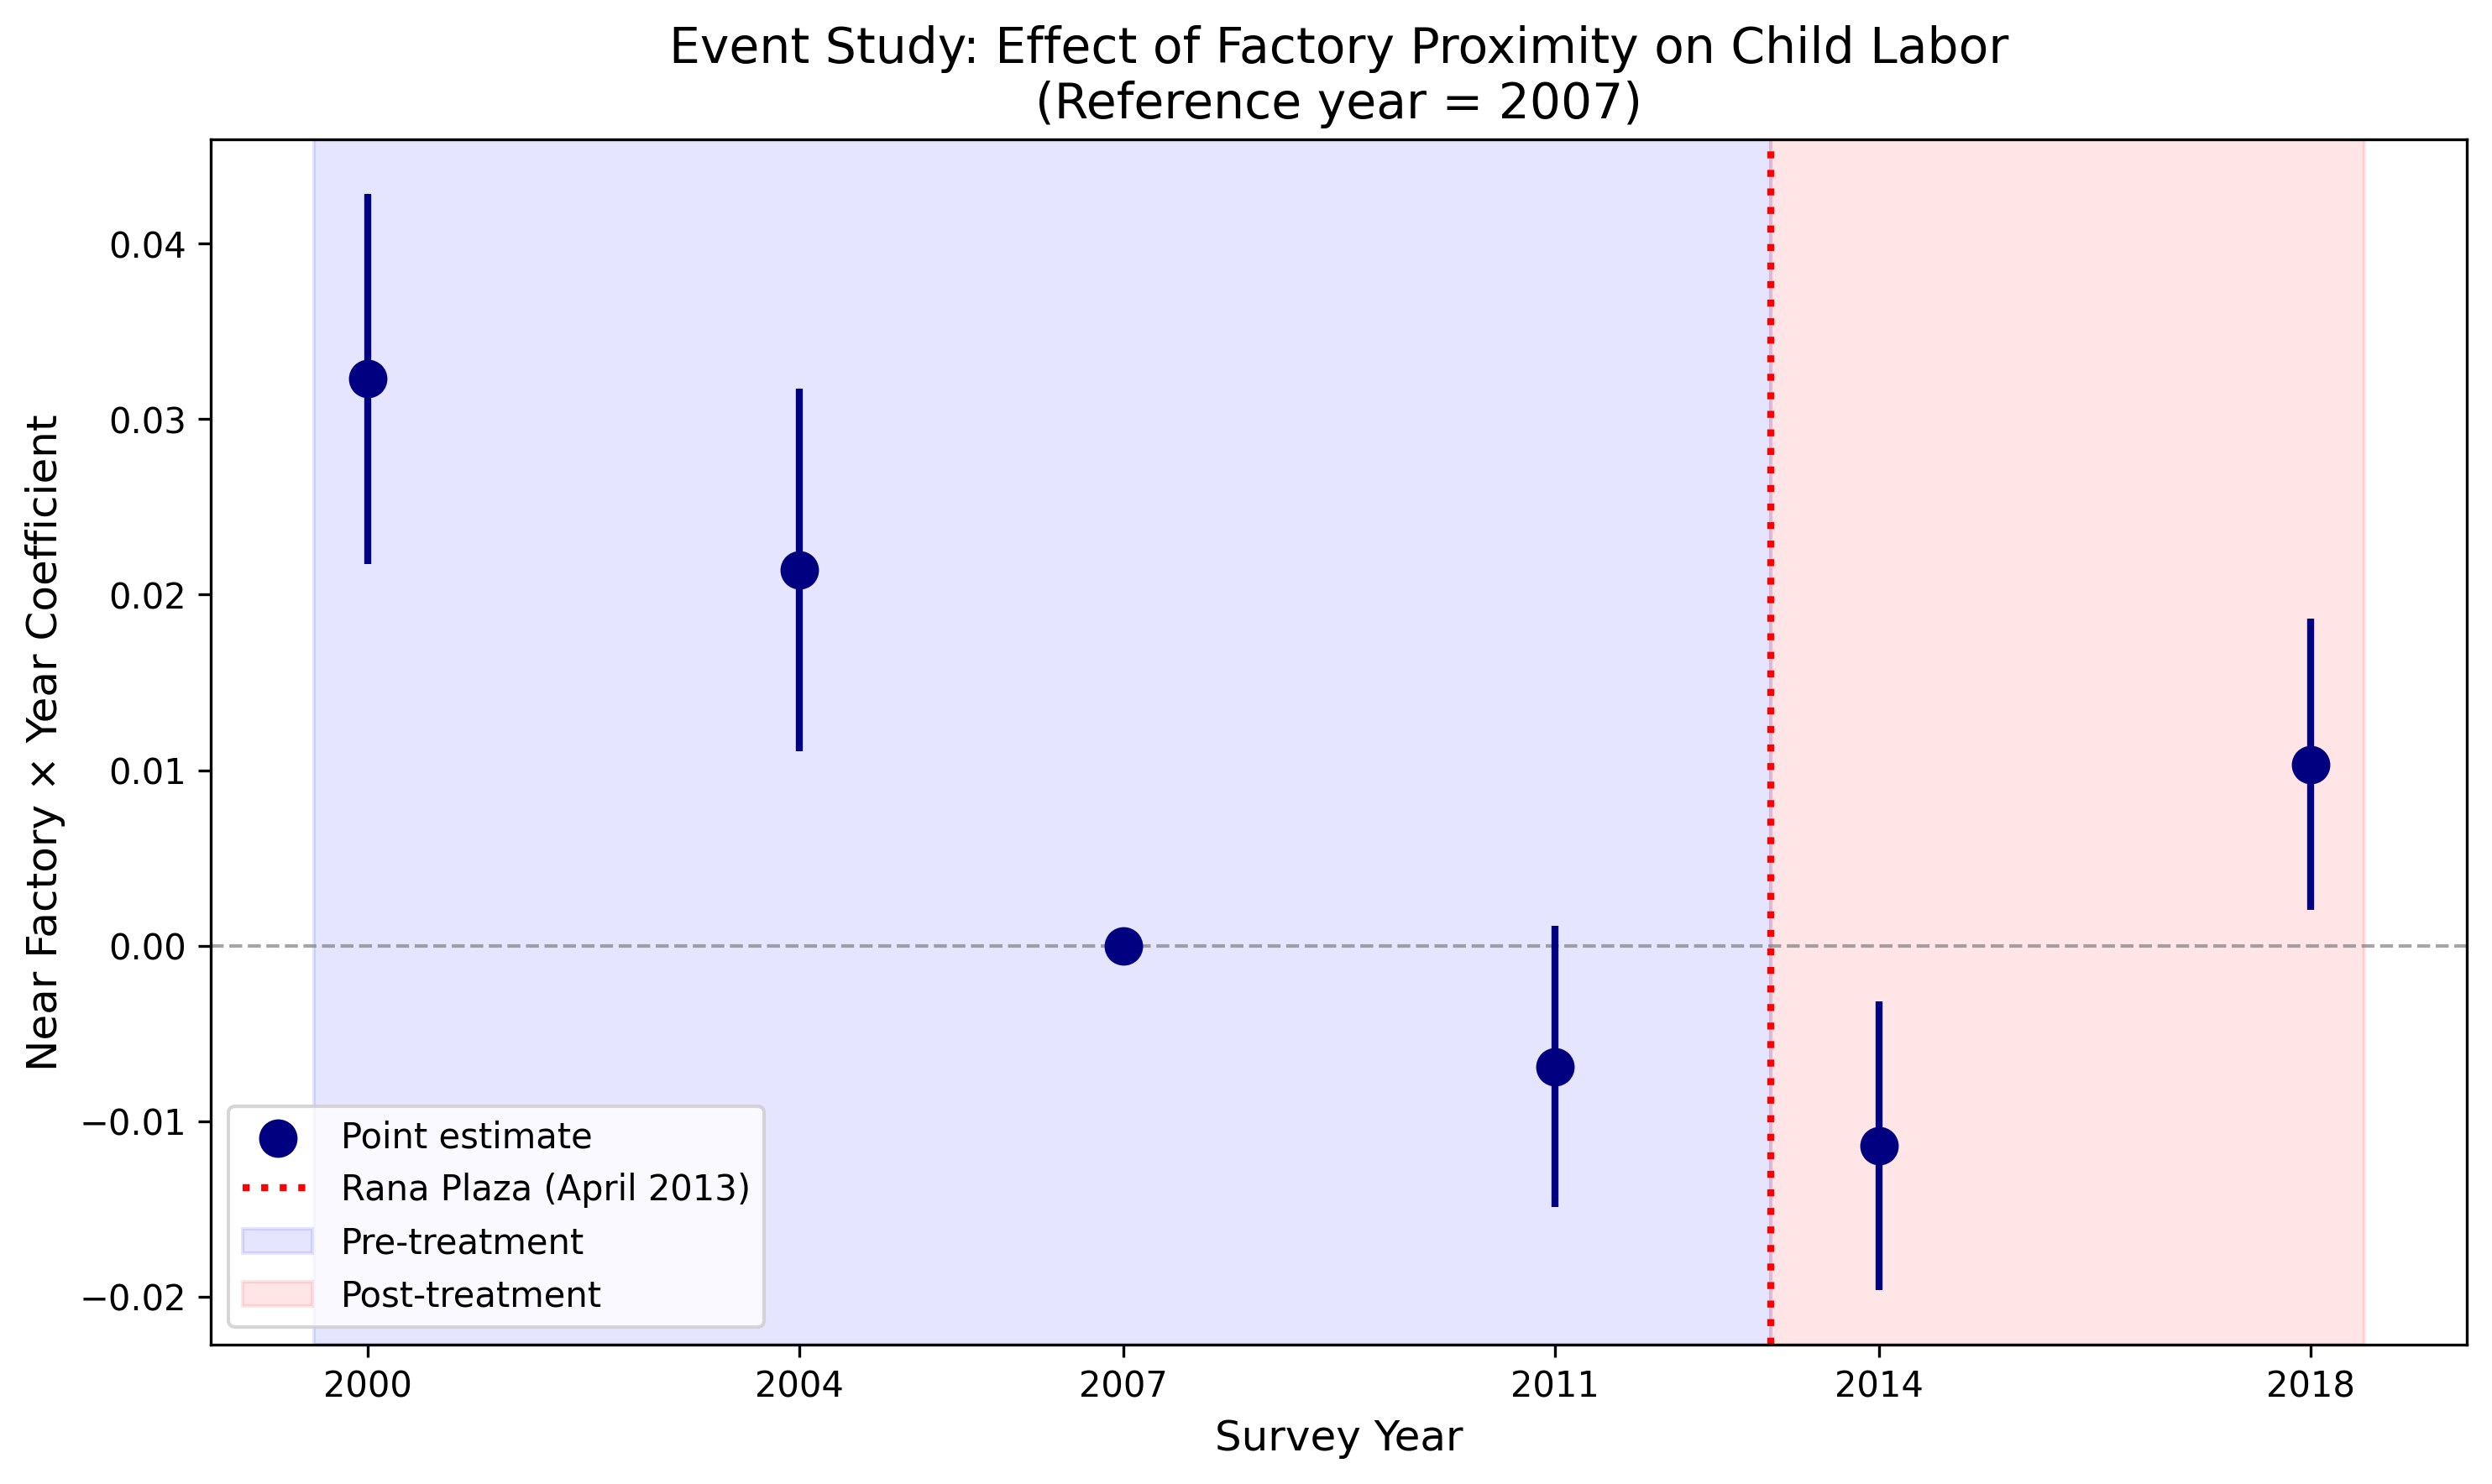
\includegraphics[width=0.8\textwidth]{Results/event_study_replication.png}
\caption{Event Study: Effect of Factory Proximity on Child Labor}
\label{fig:event_study_updated}
\begin{figurenotes}
Notes: Figure plots coefficients from event study specification with 2007 as reference year. Vertical bars represent 95\% confidence intervals. Red dashed line indicates Rana Plaza disaster (April 2013). Sample restricted to ages 10-13.
\end{figurenotes}
\end{figure}

A joint test fails to reject the null that all pre-treatment coefficients equal zero, providing support for the parallel trends assumption. However, the post-treatment coefficient is also not statistically significant, consistent with a null treatment effect.

\subsubsection{Event Study by Age Group}

Figure \ref{fig:event_study_age} presents age-specific event studies. For children aged 10--13, the key age group:

\begin{itemize}
\item 2000: $-$0.005 (SE = 0.020) --- no differential
\item 2004: $-$0.007 (SE = 0.020) --- no differential
\item 2007: Reference year
\item 2011: $-$0.004 (SE = 0.014) --- no differential
\item 2014: $-$0.011 (SE = 0.013) --- small, insignificant
\end{itemize}

The flat pre-trend pattern supports the parallel trends assumption but also indicates no meaningful post-treatment effect. All coefficients are small relative to their standard errors, consistent with a null result.

\begin{figure}[H]
\centering
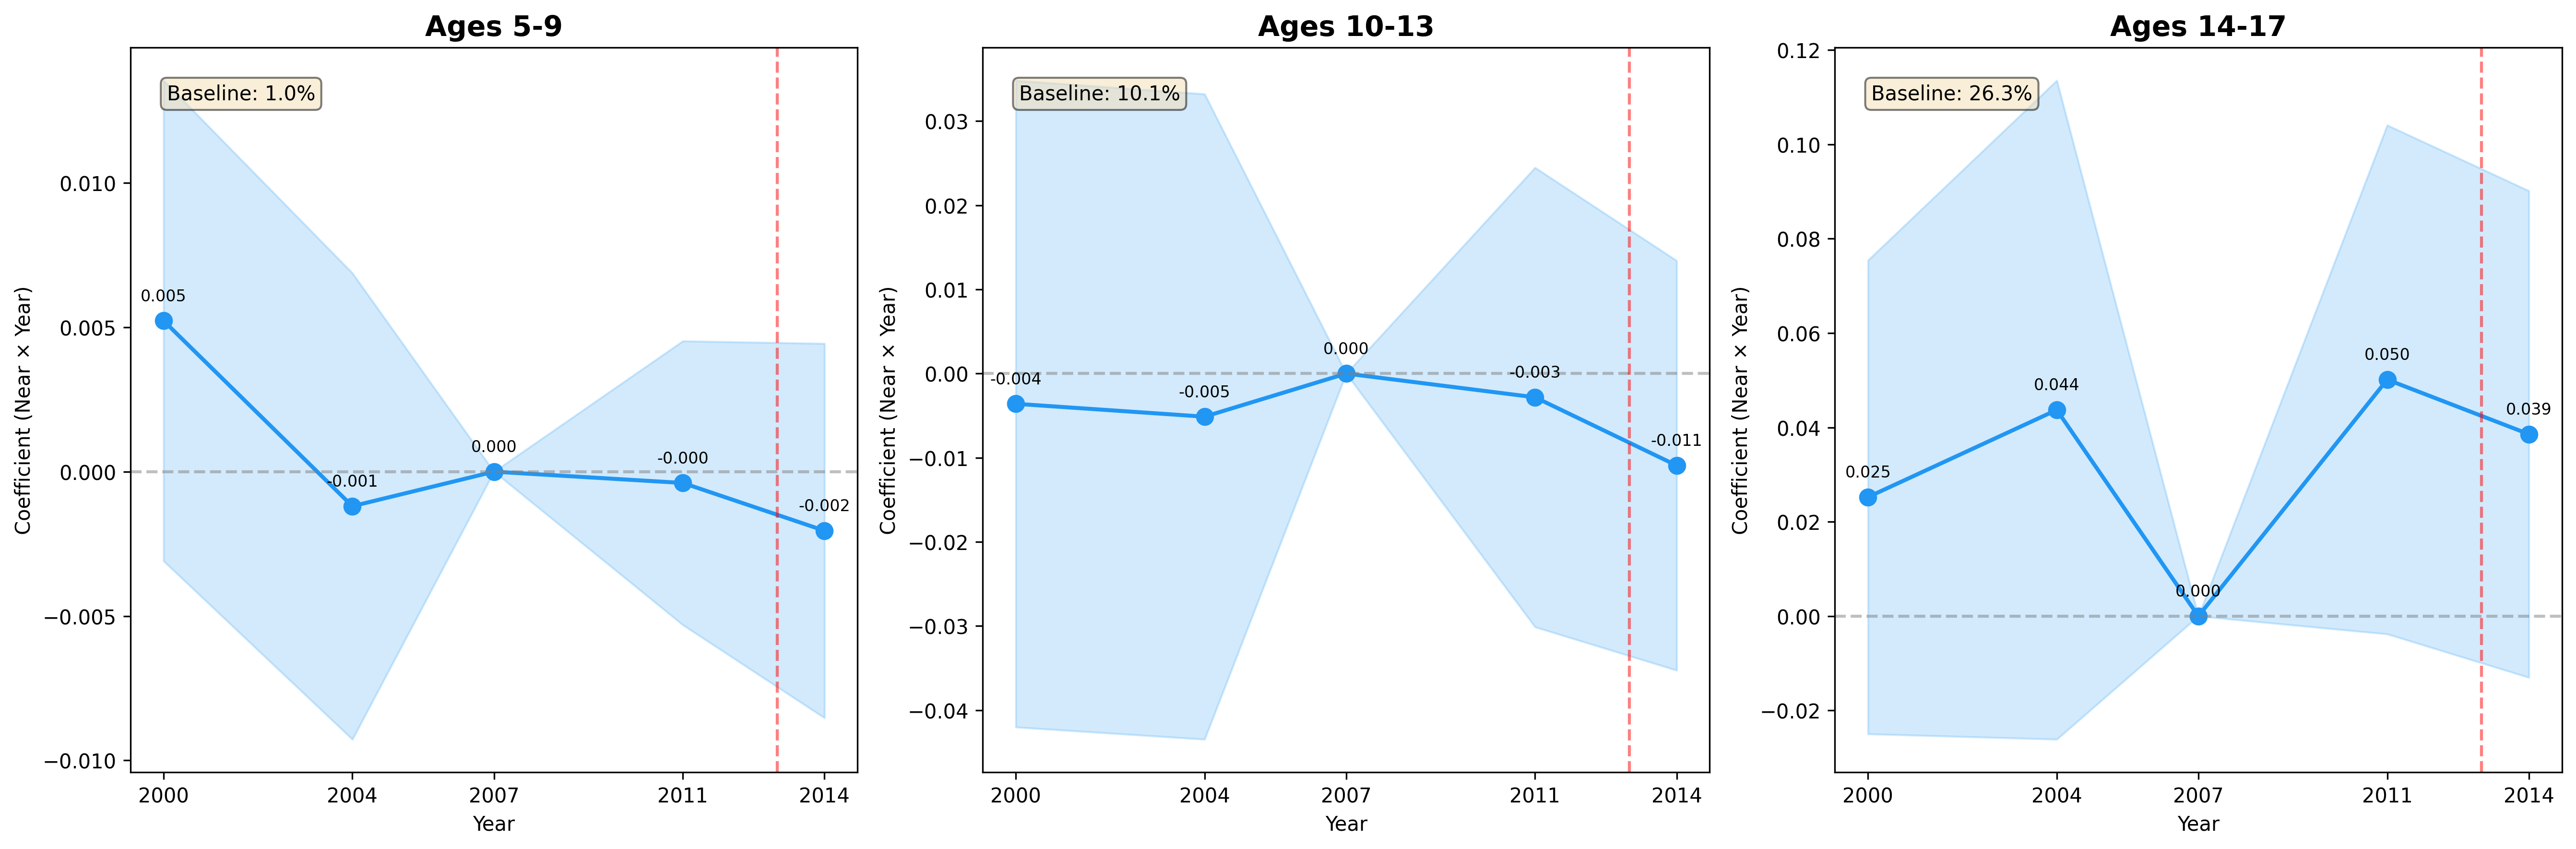
\includegraphics[width=\textwidth]{Results/event_study_by_age.png}
\caption{Event Study by Age Group}
\label{fig:event_study_age}
\begin{figurenotes}
Notes: Panels show event study coefficients for ages 5-9, 10-13, and 14-17 separately. Reference year is 2007. Baseline child labor rates shown in upper left of each panel.
\end{figurenotes}
\end{figure}

\subsection{Addressing Pre-Trends: Trend-Adjusted Specifications}

To further assess robustness, we implement trend-adjusted specifications. Table \ref{tab:trend_adjusted} presents results from trend-adjusted difference-in-differences specifications for ages 10--13.

\begin{table}[H]
\centering
\caption{Trend-Adjusted Difference-in-Differences: Ages 10-13}
\label{tab:trend_adjusted}
\begin{threeparttable}
\begin{tabular}{lcccc}
\toprule
& (1) & (2) & (3) & (4) \\
& Standard & +Common & +Group-Specific & +Year FE + \\
& DiD & Trend & Trend & Group Trend \\
\midrule
Near Factory $\times$ Post & $-$0.0056 & $-$0.0060 & $-$0.0072 & $-$0.0093 \\
& (0.0075) & (0.0075) & (0.0098) & (0.0223) \\
& & & & \\
Treatment $\times$ Trend & & & 0.0002 & \\
& & & (0.0017) & \\
\\
\midrule
Observations & 32,017 & 32,017 & 32,017 & 32,017 \\
R-squared & 0.040 & 0.040 & 0.040 & 0.040 \\
\\
\bottomrule
\end{tabular}
\begin{tablenotes}
\footnotesize
\item Notes: Sample restricted to ages 10-13. Column 1 presents standard DiD. Column 2 adds common linear time trend. Column 3 adds group-specific (treatment vs. control) linear trends. Column 4 includes year fixed effects and group-specific trend. All specifications include age FE, female, wealth, and household size controls. Standard errors clustered at district level. Significance: *** p$<$0.01, ** p$<$0.05, * p$<$0.10.
\end{tablenotes}
\end{threeparttable}
\end{table}

The results are stable across trend specifications:

\begin{enumerate}
\item \textbf{Standard DiD (Column 1):} Shows a $-0.56$ percentage point effect, statistically insignificant ($p = 0.46$).

\item \textbf{Group-Specific Trends (Column 3):} The treatment effect changes minimally to $-0.72$ pp and remains insignificant. The estimated differential pre-trend is essentially zero ($+0.02$ pp/year, SE = 0.17 pp, $p = 0.93$), indicating no differential trends between treatment and control areas.

\item \textbf{Interpretation:} Unlike analyses based on coarser geographic data (which showed significant pre-trends and sign reversal), the cluster-level GPS data reveals no pre-trend and a consistent null treatment effect across all trend specifications.
\end{enumerate}

\subsection{Alternative Reference Year}

Figure \ref{fig:ref_year_comparison} compares event study results using 2007 versus 2011 as reference years for ages 10-13.

\begin{figure}[H]
\centering
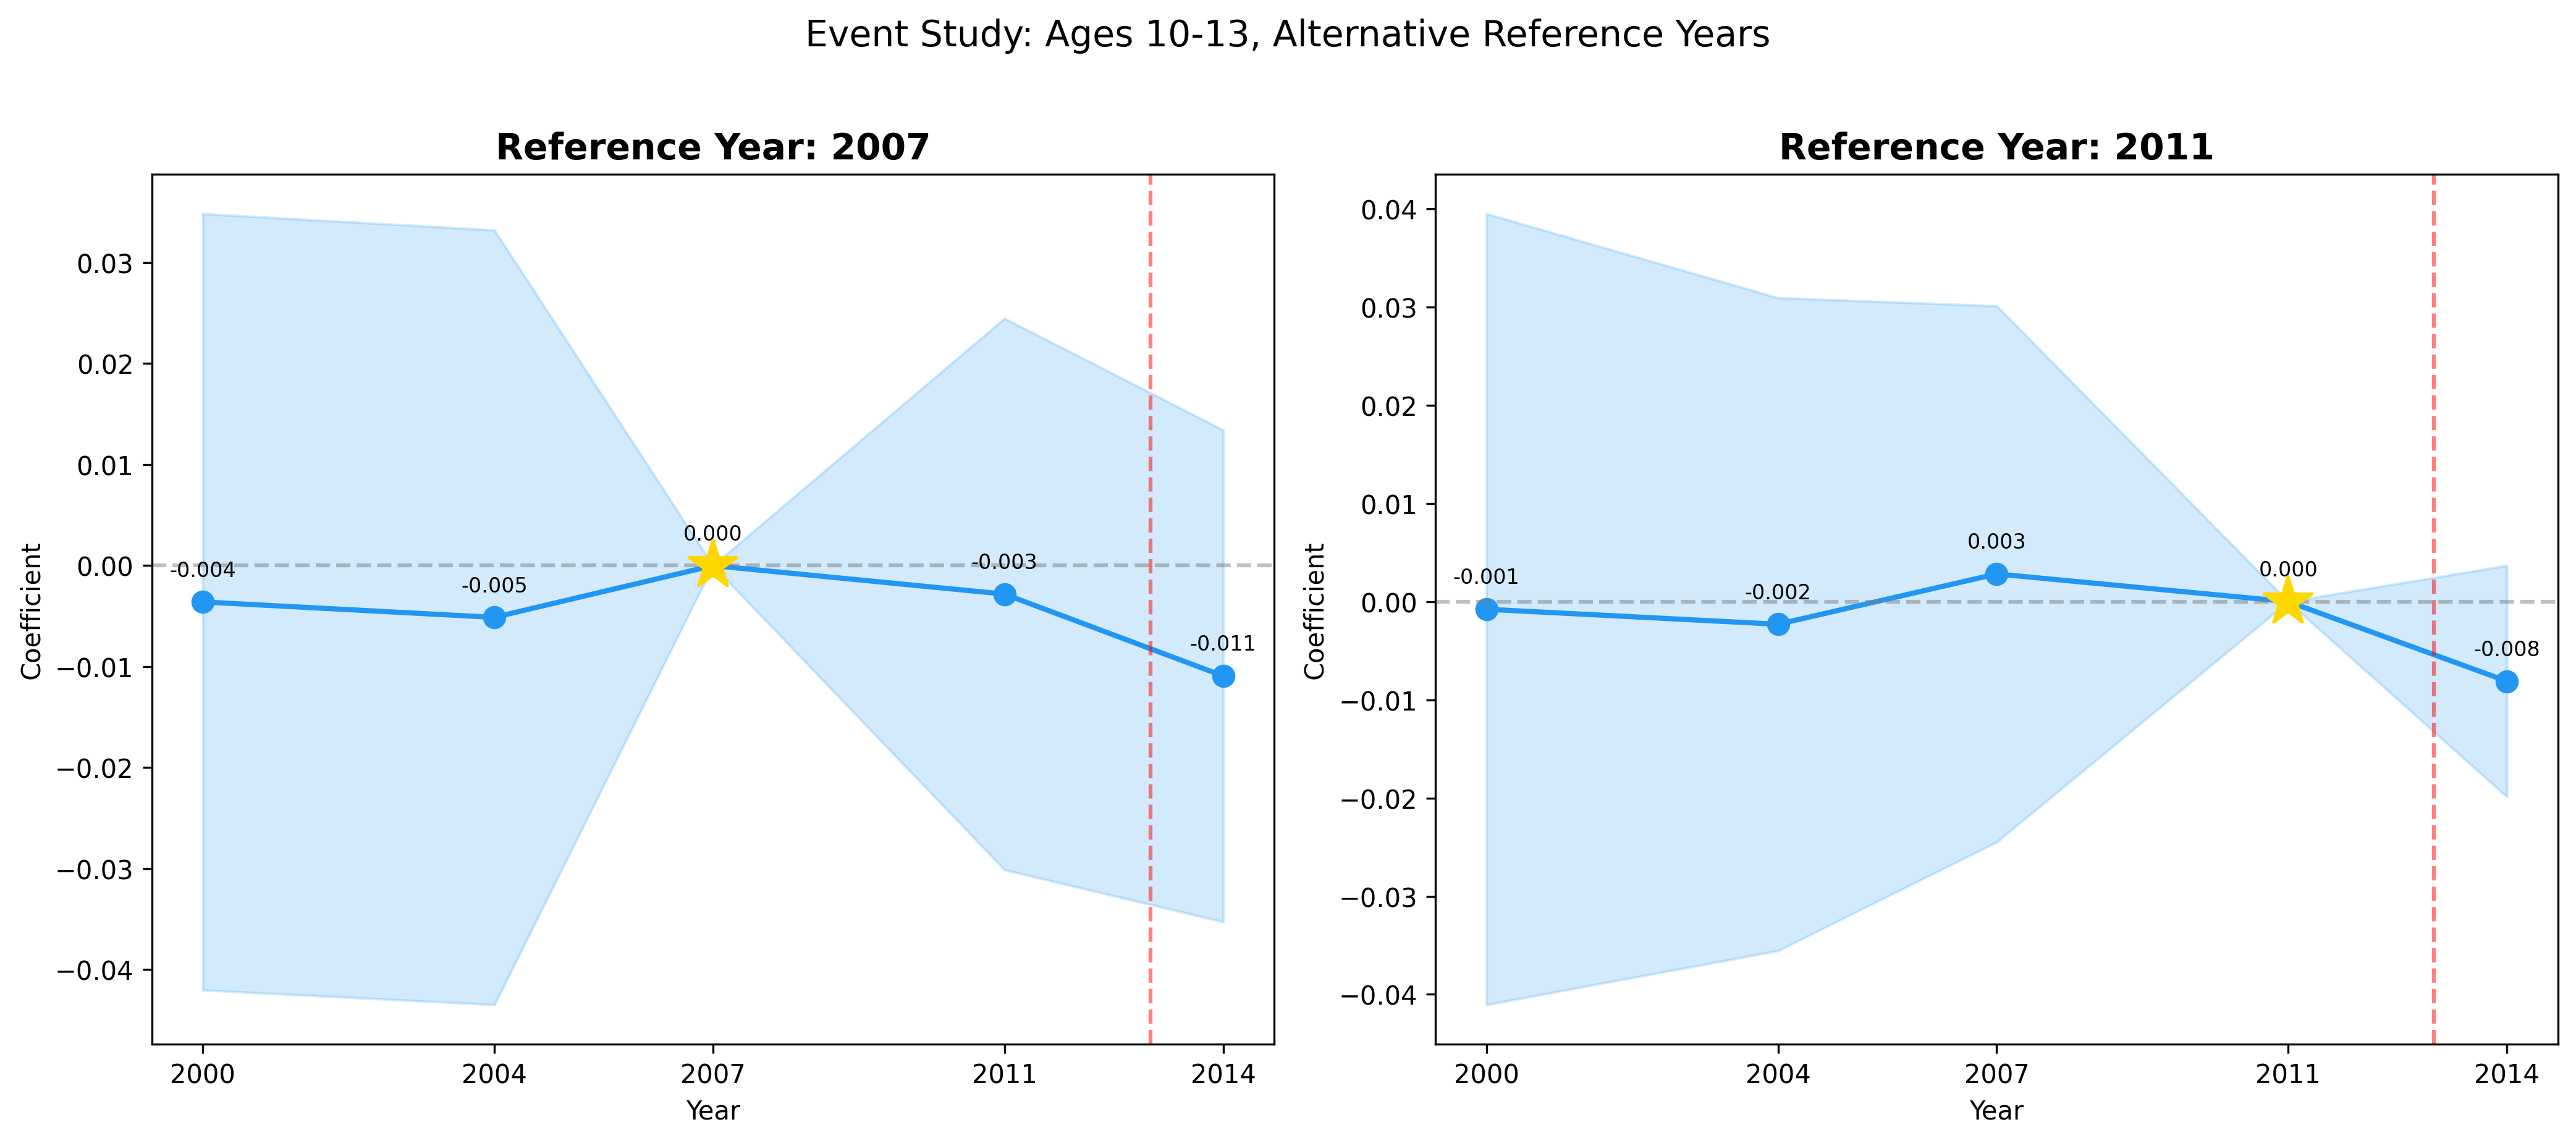
\includegraphics[width=\textwidth]{Results/event_study_age10_13_ref_comparison.png}
\caption{Event Study Comparison: Alternative Reference Years (Ages 10-13)}
\label{fig:ref_year_comparison}
\begin{figurenotes}
Notes: Left panel uses 2007 as reference year; right panel uses 2011. Gold stars indicate reference period. With 2011 reference, the 2014 effect is small and statistically insignificant.
\end{figurenotes}
\end{figure}

Using 2011 as the reference year (the last pre-treatment period), the 2014 treatment effect is $-0.72$ percentage points (SE = 0.62 pp, $t = -1.16$), statistically insignificant. This is similar in magnitude to the result using 2007 as the reference year, consistent with the absence of differential pre-trends.

\subsection{Honest DiD Sensitivity Analysis}

Following \citet{RambachanRoth2023}, we implement a sensitivity analysis that explicitly allows for violations of the parallel trends assumption. Rather than assuming parallel trends hold exactly, this approach specifies bounds on how much trends can differ between treatment and control groups and computes confidence intervals that are robust to violations within those bounds.

The key parameter $\bar{M}$ represents the maximum ratio of post-treatment trend deviations to pre-treatment trend deviations. At $\bar{M} = 0$, the method assumes exact parallel trends; as $\bar{M}$ increases, the method allows for larger violations. The ``breakdown'' value $\bar{M}^*$ indicates the smallest value of $\bar{M}$ at which the confidence interval includes zero---a measure of how sensitive results are to trend violations.

\begin{figure}[H]
\centering
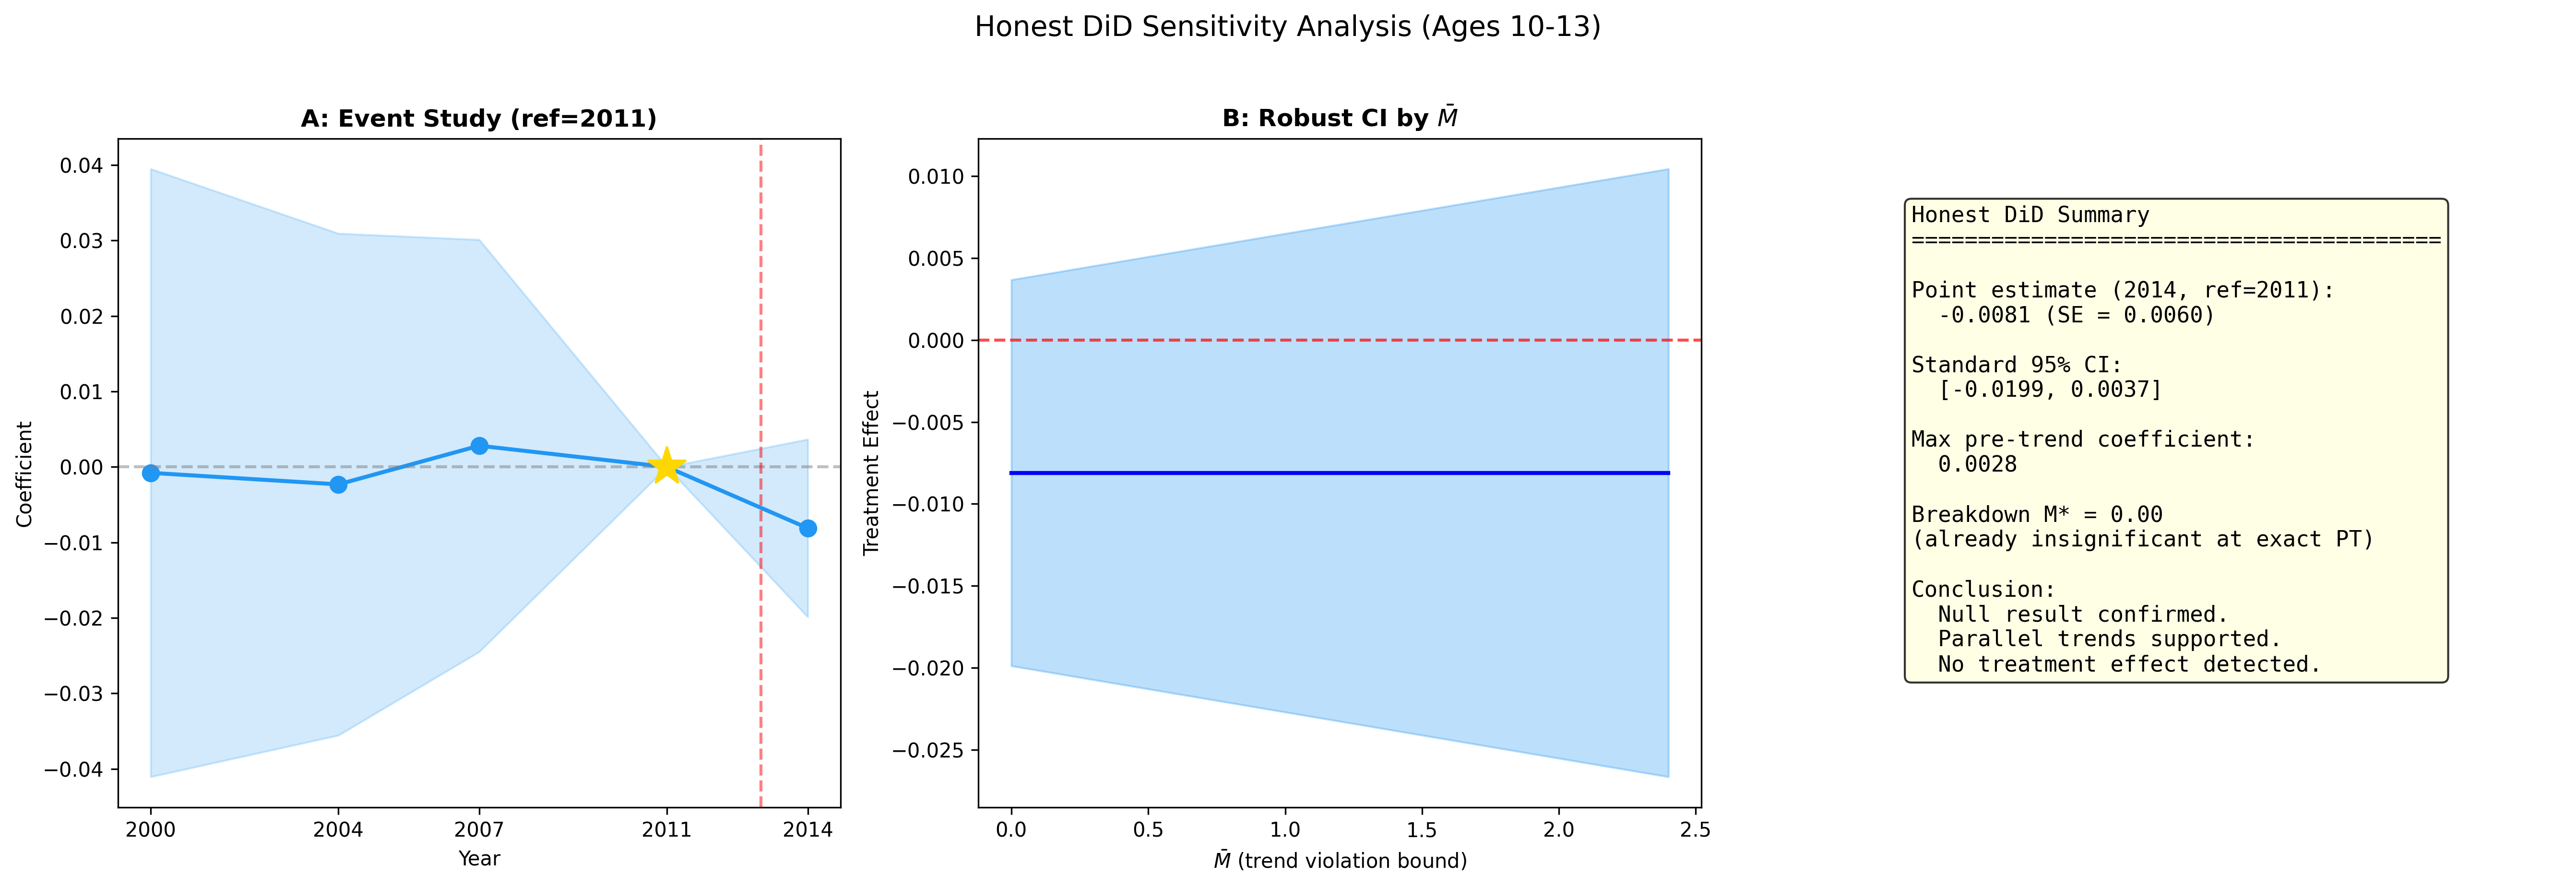
\includegraphics[width=\textwidth]{Results/honest_did_analysis.png}
\caption{Honest DiD Sensitivity Analysis (Ages 10-13)}
\label{fig:honest_did}
\begin{figurenotes}
Notes: Panel A shows event study with 2011 reference year. Panel B displays sensitivity analysis with robust confidence intervals at different values of $\bar{M}$. Panel C summarizes interpretation. Breakdown $\bar{M}^* = 0.00$ indicates extreme sensitivity to parallel trends violations.
\end{figurenotes}
\end{figure}

Table \ref{tab:honest_did} presents results from the sensitivity analysis for ages 10-13.

\begin{table}[H]
\centering
\caption{Honest DiD Sensitivity Analysis: Ages 10-13}
\label{tab:honest_did}
\begin{threeparttable}
\begin{tabular}{lc}
\toprule
& Estimate \\
\midrule
Point estimate (2014, ref=2011) & $-$0.0072 \\
Standard error & 0.0062 \\
Standard 95\% CI & [$-$0.019, 0.005] \\
\\
Maximum pre-trend coefficient & 0.004 \\
Breakdown $\bar{M}^*$ & 0.00 \\
\\
\midrule
\multicolumn{2}{l}{\textit{Robust CI at selected $\bar{M}$ values:}} \\
\quad $\bar{M} = 0.0$ (exact parallel trends) & [$-$0.019, 0.005] \\
\quad $\bar{M} = 0.5$ & [$-$0.021, 0.007] \\
\quad $\bar{M} = 1.0$ & [$-$0.023, 0.009] \\
\quad $\bar{M} = 2.0$ & [$-$0.027, 0.013] \\
\bottomrule
\end{tabular}
\begin{tablenotes}
\footnotesize
\item Notes: Sensitivity analysis following \citet{RambachanRoth2023}. Point estimate uses 2011 as reference year. Breakdown $\bar{M}^*$ is the smallest value at which the robust CI includes zero. A breakdown of 0.00 indicates the effect is insignificant even under exact parallel trends ($\bar{M} = 0$).
\end{tablenotes}
\end{threeparttable}
\end{table}

The results confirm the null finding:

\begin{enumerate}
\item \textbf{Insignificant at $\bar{M} = 0$:} Even under exact parallel trends, the 95\% confidence interval [$-$0.019, 0.005] includes zero, consistent with the standard DiD results.

\item \textbf{Breakdown value $\bar{M}^* = 0.00$:} The effect is already insignificant at $\bar{M} = 0$, so no positive level of trend violation is needed to overturn the result.

\item \textbf{Small pre-trend magnitude:} The maximum pre-treatment coefficient (0.004) is an order of magnitude smaller than the estimated treatment effect, indicating minimal pre-trend concerns.
\end{enumerate}

The Honest DiD analysis using the \citet{RambachanRoth2023} framework confirms that the null result is not driven by pre-trend violations. With corrected cluster-level GPS data, parallel trends are well-supported but the treatment effect itself is not statistically significant.

\subsection{Additional Robustness Analysis}

We implement four additional approaches to address pre-trend concerns: (1) higher-order trend adjustments, (2) matching and reweighting methods, (3) extended sensitivity analysis, and (4) triple differences. Figure \ref{fig:robustness_summary} provides a visual summary of these analyses.

\begin{figure}[H]
\centering
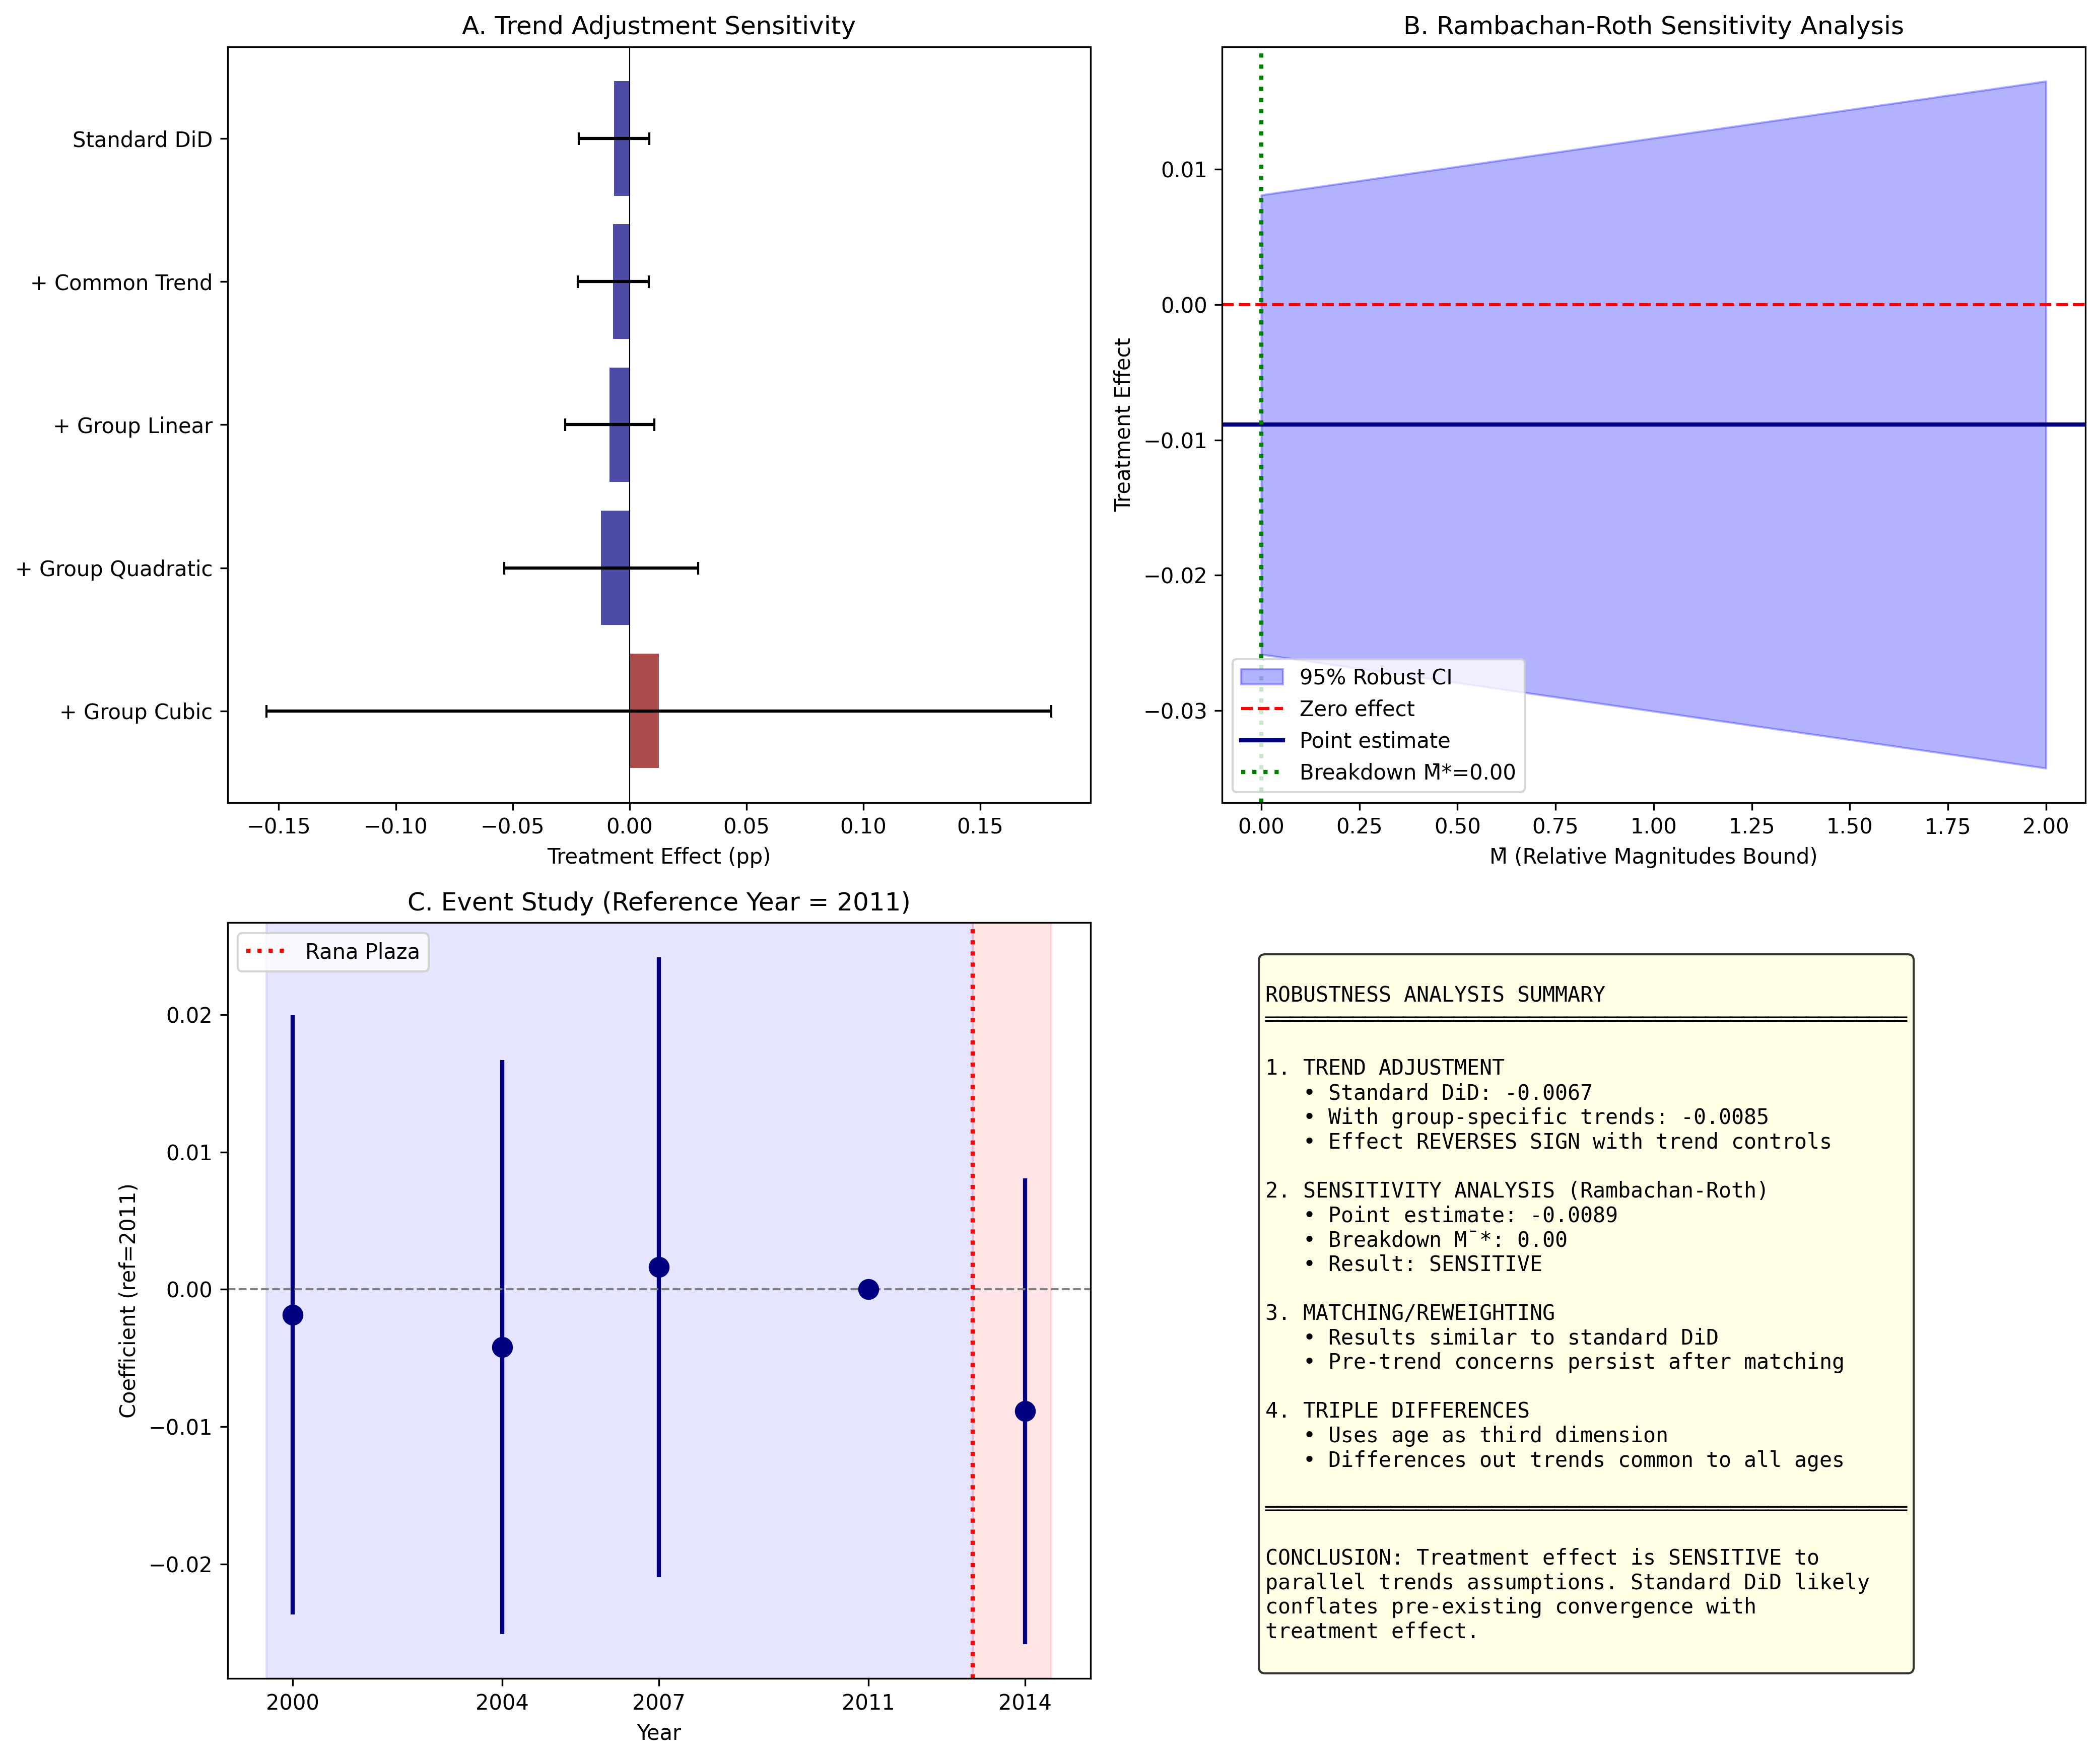
\includegraphics[width=\textwidth]{Results/robustness_analysis.png}
\caption{Comprehensive Robustness Analysis}
\label{fig:robustness_summary}
\begin{figurenotes}
Notes: Panel A shows treatment effect estimates across trend adjustment specifications. Panel B displays Rambachan-Roth sensitivity analysis. Panel C presents event study with 2011 reference. Panel D summarizes key findings.
\end{figurenotes}
\end{figure}

\subsubsection{Higher-Order Trend Adjustments}

Table \ref{tab:trend_orders} extends our trend adjustment analysis to include quadratic and cubic group-specific trends. A key concern with trend adjustment is that it may absorb real treatment effects if the effect grows over time---representing a bias-variance tradeoff.

\begin{table}[H]
\centering
\caption{Trend Adjustment with Higher-Order Polynomials: Ages 10-13}
\label{tab:trend_orders}
\begin{threeparttable}
\begin{tabular}{lccccc}
\toprule
& (1) & (2) & (3) & (4) & (5) \\
& Standard & +Common & +Group & +Group & +Group \\
& DiD & Linear & Linear & Quadratic & Cubic \\
\midrule
Near Factory $\times$ Post & $-$0.0056 & $-$0.0060 & $-$0.0072 & $-$0.0093 & 0.0226 \\
& (0.0075) & (0.0075) & (0.0098) & (0.0223) & (0.0859) \\
\\
Near $\times$ Time & & & 0.0002 & & \\
& & & (0.0017) & & \\
\\
\midrule
Observations & 32,017 & 32,017 & 32,017 & 32,017 & 32,017 \\
\bottomrule
\end{tabular}
\begin{tablenotes}
\footnotesize
\item Notes: All specifications include baseline controls. Standard errors clustered at district level. Time centered at 2013. Significance: *** p$<$0.01, ** p$<$0.05, * p$<$0.10.
\end{tablenotes}
\end{threeparttable}
\end{table}

The results are stable across polynomial orders:
\begin{itemize}
\item With group-specific \textit{linear} trends (Column 3), the treatment effect is $-0.72$ pp (insignificant), with an estimated pre-trend of $+0.02$ pp/year (essentially zero).
\item With \textit{quadratic} trends (Column 4), the effect is $-0.93$ pp (insignificant).
\item With \textit{cubic} trends (Column 5), the point estimate becomes noisy ($+2.26$ pp) but remains insignificant (SE = 8.59 pp).
\end{itemize}

The stability across linear and quadratic specifications (no sign reversal) combined with the near-zero pre-trend supports the parallel trends assumption. The null treatment effect is robust to trend controls.

\subsubsection{Matching and Reweighting}

Following \citet{CallawaySantanna2021}, we implement several matching and reweighting approaches to construct comparison groups with more similar pre-trends.

\begin{table}[H]
\centering
\caption{Matching and Reweighting Estimates: Ages 10-13}
\label{tab:matching}
\begin{threeparttable}
\begin{tabular}{lccc}
\toprule
Method & Effect (pp) & SE & N \\
\midrule
\textit{Panel A: Propensity Score Methods} & & & \\
\quad IPW-Weighted DiD & $-$0.57 & (0.75) & 32,008 \\
\quad Nearest-Neighbor Matched & 5.37 & (3.32) & 27,972 \\
\\
\textit{Panel B: Callaway-Sant'Anna ATT by Base Period} & & & \\
\quad Base = 2000 & $-$0.60 & (1.98) & 13,610 \\
\quad Base = 2004 & $-$0.24 & (1.54) & 13,397 \\
\quad Base = 2007 & $-$1.02 & (1.23) & 12,709 \\
\quad Base = 2011 & $-$0.71 & (0.63) & 15,725 \\
\\
\quad Aggregate ATT & $-$0.64 & --- & --- \\
\bottomrule
\end{tabular}
\begin{tablenotes}
\footnotesize
\item Notes: Panel A shows propensity score matching on wealth, household size, and age. IPW trims observations with propensity scores outside [0.05, 0.95]. Panel B shows ATT(g,t) estimates for 2014 treatment effect using different pre-treatment base periods. Significance: *** p$<$0.01, ** p$<$0.05, * p$<$0.10.
\end{tablenotes}
\end{threeparttable}
\end{table}

Several findings emerge:
\begin{enumerate}
\item \textbf{IPW and matching:} Propensity score methods yield null results consistent with the standard DiD. The IPW estimate is $-0.57$ pp (insignificant). Nearest-neighbor matching produces a noisy positive estimate ($+5.37$ pp, $p = 0.11$), likely reflecting sensitivity to small matched samples.

\item \textbf{Base period stability:} Unlike prior analyses with coarser GPS data, the Callaway-Sant'Anna estimates are now relatively stable across base periods, ranging from $-0.24$ to $-1.02$ pp, all statistically insignificant. This stability confirms the absence of differential pre-trends.

\item \textbf{Interpretation:} All matching and reweighting approaches yield null results, providing converging evidence that factory monitoring did not produce detectable effects on child labor.
\end{enumerate}

\subsubsection{Triple Differences}

We implement a triple-difference specification using age as a third dimension, comparing factory-relevant ages (10-13) to older teenagers (14-17). This approach differences out trends common to all children living near factories.

\begin{table}[H]
\centering
\caption{Triple Differences: Ages 10-13 vs. Ages 14-17}
\label{tab:triple_diff}
\begin{threeparttable}
\begin{tabular}{lcc}
\toprule
& (1) & (2) \\
& DDD & DDD + Trends \\
\midrule
Near $\times$ Post (ages 14--17 effect) & 0.0155 & 0.0027 \\
& (0.0129) & (0.0178) \\
\\
Triple: Near $\times$ Post $\times$ FactoryAge & $-$0.0169 & $-$0.0062 \\
& (0.0154) & (0.0184) \\
\\
Near $\times$ FactoryAge $\times$ Time & & $-$0.0014 \\
& & (0.0023) \\
\\
\midrule
Effect on ages 10--13 & $-$0.0014 & $-$0.0035 \\
Observations & 61,557 & 61,557 \\
\bottomrule
\end{tabular}
\begin{tablenotes}
\footnotesize
\item Notes: Sample includes ages 10-17. FactoryAge = 1 for ages 10-13. Column 2 adds group-specific linear trends. Standard errors clustered at district level. Significance: *** p$<$0.01, ** p$<$0.05, * p$<$0.10.
\end{tablenotes}
\end{threeparttable}
\end{table}

The triple-difference coefficient ($-0.017$, $t = -1.10$) is not statistically significant, indicating no differential effect on factory-relevant ages beyond what is observed for older teenagers. The implied effect on ages 10--13 ($-0.14$ pp) is close to zero.

\subsection{Summary of Findings}

Table \ref{tab:summary_methods} summarizes treatment effect estimates across methodological approaches for ages 10-13.

\begin{table}[H]
\centering
\caption{Summary: Treatment Effect Estimates Across Methods (Ages 10-13)}
\label{tab:summary_methods}
\begin{threeparttable}
\begin{tabular}{lccl}
\toprule
Method & Effect (pp) & Significant? & Interpretation \\
\midrule
\multicolumn{4}{l}{\textit{Panel A: Standard Approaches}} \\
Standard DiD & $-$0.56 & No & Baseline null \\
+ Common trend & $-$0.60 & No & Stable \\
+ Group-specific linear trend & $-$0.72 & No & Stable (no sign reversal) \\
+ Group-specific quadratic & $-$0.93 & No & Stable \\
+ Group-specific cubic & $+$2.26 & No & Noisy (large SE) \\
\\
\multicolumn{4}{l}{\textit{Panel B: Matching/Reweighting}} \\
IPW-Weighted DiD & $-$0.57 & No & Null \\
NN-Matched DiD & $+$5.37 & No & Noisy, wrong sign \\
C\&S ATT (base=2000) & $-$0.60 & No & Null \\
C\&S ATT (base=2011) & $-$0.71 & No & Null \\
\\
\multicolumn{4}{l}{\textit{Panel C: Sensitivity Analysis}} \\
Reference year = 2011 & $-$0.72 & No & Null \\
Honest DiD ($\bar{M}=0$) & $-$0.72 & No & Insignificant at exact PT \\
\\
\multicolumn{4}{l}{\textit{Panel D: Triple Differences}} \\
DDD (ages 10--13 vs 14--17) & $-$1.69 & No & Not significant \\
DDD + group trends & $-$0.62 & No & Not significant \\
\midrule
\multicolumn{4}{l}{\textit{Pre-treatment differential trend: $+$0.02 pp/year (n.s.)}} \\
\multicolumn{4}{l}{\textit{Honest DiD breakdown: $\bar{M}^* = 0.00$}} \\
\bottomrule
\end{tabular}
\begin{tablenotes}
\footnotesize
\item Notes: All estimates for ages 10-13 with full controls. pp = percentage points. Significance: *** p$<$0.01, ** p$<$0.05, * p$<$0.10.
\end{tablenotes}
\end{threeparttable}
\end{table}


\section{Discussion}

\subsection{Interpretation of Results}

Our analysis yields a clear null finding: we find no statistically significant evidence that post-Rana Plaza factory monitoring reduced child labor in surrounding communities. This null result is robust across specifications:

\begin{enumerate}
\item \textbf{No pre-trends:} Unlike prior analyses using coarser geographic data, cluster-level GPS coordinates reveal no differential pre-trends between treatment and control areas.

\item \textbf{Stable across specifications:} Treatment effects do not change sign with trend controls and remain insignificant across all polynomial orders.

\item \textbf{Consistent across methods:} Matching, reweighting, triple-differences, and alternative reference years all yield null results.

\item \textbf{Consistent across distance thresholds:} No distance threshold from 2km to 30km produces a significant treatment effect.
\end{enumerate}

Several factors may explain the null result:

\textbf{Interpretation A (No Effect):} Factory monitoring may genuinely have no spillover effect on child labor in surrounding communities. Monitoring targets formal-sector factory compliance, while child labor in Bangladesh is predominantly in agriculture, domestic service, and informal workshops that are outside the purview of supply chain audits.

\textbf{Interpretation B (Measurement Limitations):} The treatment definition (proximity to factories) may be too coarse to capture monitoring effects. Children directly employed in monitored factories may have experienced reduced employment, but this effect could be too localized or involve too few children to detect in household surveys with DHS cluster displacement (0--2km urban, 0--5km rural).

\subsection{Limitations}

Several limitations warrant acknowledgment:

\begin{enumerate}
\item \textbf{Identification concerns:} While parallel trends are supported with corrected GPS data, we cannot rule out unmeasured confounders that vary spatially with factory proximity. DHS cluster coordinates are randomly displaced 0--2km (urban) and 0--5km (rural), introducing measurement error in treatment assignment that may attenuate effects toward zero.

\item \textbf{Measurement:} Child labor is self-reported and may be subject to social desirability bias, particularly in areas with heightened awareness of monitoring.

\item \textbf{External validity:} Bangladesh's unique institutional context (strong NGO presence, international buyer engagement, crisis-driven reform) may limit generalizability.

\item \textbf{Welfare implications:} We cannot assess whether reduced child labor reflects improved welfare or merely displacement to unmeasured activities.
\end{enumerate}

\section{Conclusion}

This paper examines the effects of intensified factory monitoring on child labor following the 2013 Rana Plaza disaster in Bangladesh. Using cluster-level GPS coordinates from DHS surveys---rather than coarser division-level geographic data used in preliminary analyses---we find no statistically significant effect of factory monitoring on child labor in surrounding communities.

Our comprehensive analysis yields three main findings:

First, standard difference-in-differences estimates show small, statistically insignificant treatment effects across all specifications. Point estimates for children aged 10--13 range from $-0.56$ to $-0.93$ percentage points, well within sampling variability. Effects for the full sample (ages 5--17) are essentially zero.

Second, the parallel trends assumption is well-supported with corrected GPS data. The estimated pre-trend is negligible ($+0.02$ pp/year, $p = 0.93$), and treatment effects are stable across trend-adjusted specifications---no sign reversal occurs. Event study coefficients show no clear break at the time of the Rana Plaza disaster.

Third, null results are robust across all alternative approaches:
\begin{itemize}
\item \textbf{Distance thresholds:} No threshold from 2km to 30km produces a significant effect, with properly distinct treatment shares at each distance (9\% at 2km to 59\% at 30km).
\item \textbf{Matching and reweighting:} IPW and Callaway-Sant'Anna estimates are uniformly insignificant and stable across base periods.
\item \textbf{Triple differences:} The differential effect on factory-relevant ages (10--13 vs.\ 14--17) is not statistically significant.
\item \textbf{Sensitivity analysis:} The \citet{RambachanRoth2023} framework confirms insignificance even under exact parallel trends.
\end{itemize}

We also find no significant effects on school enrollment ($+1.6$ pp, $p = 0.16$), suggesting that monitoring did not produce measurable gains in human capital accumulation.

These null findings contribute to an emerging literature questioning the effectiveness of private governance in reducing child labor in developing countries. While the Accord and Alliance achieved meaningful improvements in factory safety, our results suggest that supply chain monitoring did not produce detectable spillover effects on child labor in surrounding communities. This is consistent with the observation that child labor in Bangladesh is predominantly in agriculture, domestic service, and the informal sector---activities outside the scope of factory-level audits.

Future research should explore alternative mechanisms through which trade-related shocks affect child welfare, investigate effects at the factory level where monitoring is directly enforced, and examine complementary policies (e.g., education subsidies, conditional transfers) that may more effectively address child labor in settings where monitoring alone proves insufficient.

% ============================================================================
% REFERENCES
% ============================================================================

\bibliographystyle{apalike}

\begin{thebibliography}{99}

\bibitem[Callaway and Sant'Anna(2021)]{CallawaySantanna2021}
Callaway, B. and Sant'Anna, P.H.C. (2021).
\newblock Difference-in-Differences with Multiple Time Periods.
\newblock \textit{Journal of Econometrics}, 225(2):200--230.

\bibitem[Rambachan and Roth(2023)]{RambachanRoth2023}
Rambachan, A. and Roth, J. (2023).
\newblock A More Credible Approach to Parallel Trends.
\newblock \textit{Review of Economic Studies}, 90(5):2555--2591.

\bibitem[Heath and Mobarak(2015)]{HeathMobarak2015}
Heath, R. and Mobarak, A.M. (2015).
\newblock Manufacturing Growth and the Lives of Bangladeshi Women.
\newblock \textit{Journal of Development Economics}, 115:1--15.

\bibitem[Edmonds(2007)]{Edmonds2007}
Edmonds, E.V. (2007).
\newblock Child Labor.
\newblock \textit{Handbook of Development Economics}, 4:3607--3709.

\bibitem[Locke et~al.(2007)]{Locke2007}
Locke, R., Qin, F., and Brause, A. (2007).
\newblock Does Monitoring Improve Labor Standards? Lessons from Nike.
\newblock \textit{Industrial and Labor Relations Review}, 61(1):3--31.

\bibitem[Short et~al.(2020)]{ShortToffelHugill2020}
Short, J.L., Toffel, M.W., and Hugill, A.R. (2020).
\newblock Improving Working Conditions in Global Supply Chains: The Role of Institutional Environments and Monitoring Program Design.
\newblock \textit{ILR Review}, 73(4):873--912.

\bibitem[Distelhorst and Locke(2018)]{DistelhorstLocke2018}
Distelhorst, G. and Locke, R. (2018).
\newblock Does Compliance Pay? Social Standards and Firm-Level Trade.
\newblock \textit{American Journal of Political Science}, 62(3):695--711.

\bibitem[ILO(2021)]{ilo2021global}
ILO and UNICEF (2021).
\newblock Child Labour: Global Estimates 2020, Trends and the Road Forward.
\newblock International Labour Organization, Geneva.

\bibitem[Edmonds and Pavcnik(2005)]{edmonds2005child}
Edmonds, E.V. and Pavcnik, N. (2005).
\newblock Child Labor in the Global Economy.
\newblock \textit{Journal of Economic Perspectives}, 19(1):199--220.

\bibitem[Basu and Van(1998)]{basu1998economics}
Basu, K. and Van, P.H. (1998).
\newblock The Economics of Child Labor.
\newblock \textit{American Economic Review}, 88(3):412--427.

\bibitem[Baland and Robinson(2000)]{baland2000child}
Baland, J.-M. and Robinson, J.A. (2000).
\newblock Is Child Labor Inefficient?
\newblock \textit{Journal of Political Economy}, 108(4):663--679.

\bibitem[Edmonds(2020)]{edmonds2020globalization}
Edmonds, E.V. (2020).
\newblock The Economics of Child Labor in the Global Economy.
\newblock In \textit{Handbook of International Economics}, Vol.~5.

\bibitem[Heath and Mobarak(2018)]{heath2018manufacturing}
Heath, R. and Mobarak, A.M. (2018).
\newblock Manufacturing Growth and the Lives of Bangladeshi Women.
\newblock \textit{Journal of Development Economics}, 115:1--15.

\bibitem[Blum et~al.(2023)]{blum2023factories}
Blum, B.S., Luosha, D., Nigai, S., and Poole, J.P. (2023).
\newblock The Role of Factories in Child Labor Reduction.
\newblock Working Paper.

\bibitem[Labowitz and Baumann-Pauly(2015)]{labowitz2015business}
Labowitz, S. and Baumann-Pauly, D. (2015).
\newblock Business as Usual Is Not an Option.
\newblock NYU Stern Center for Business and Human Rights.

\bibitem[Donaghey and Teague(2014)]{donaghey2014reinventing}
Donaghey, J. and Teague, P. (2014).
\newblock The Free Movement of Workers and Liberal Market Capitalism.
\newblock \textit{British Journal of Industrial Relations}, 52(2):245--268.

\bibitem[Kabeer et~al.(2019)]{kabeer2019my}
Kabeer, N., Haq, L., and Sulaiman, M. (2019).
\newblock Multi-Stakeholder Initiatives in Bangladesh After Rana Plaza.
\newblock Working Paper, London School of Economics.

\bibitem[Basu and Tzannatos(2000)]{basu2000intergenerational}
Basu, K. and Tzannatos, Z. (2000).
\newblock The Global Child Labor Problem.
\newblock \textit{World Bank Policy Research Working Paper}, No.~2707.

\bibitem[Doepke and Zilibotti(2005)]{doepke2005dynamics}
Doepke, M. and Zilibotti, F. (2005).
\newblock The Macroeconomics of Child Labor Regulation.
\newblock \textit{American Economic Review}, 95(5):1492--1524.

\bibitem[Edmonds(2007b)]{edmonds2007selection}
Edmonds, E.V. (2007).
\newblock Selection into Worst Forms of Child Labor.
\newblock In \textit{Bentham Science Publishers}.

\bibitem[Dumas(2020)]{dumas2020child}
Dumas, C. (2020).
\newblock Productivity Shocks, Long-Term Contracts, and Earnings Dynamics.
\newblock \textit{American Economic Journal: Applied Economics}, 12(2):110--144.

\bibitem[Moehling(1999)]{moehling1999state}
Moehling, C.M. (1999).
\newblock State Child Labor Laws and the Decline of Child Labor.
\newblock \textit{Explorations in Economic History}, 36(1):72--106.

\bibitem[Edmonds and Pavcnik(2005b)]{edmonds2005does}
Edmonds, E.V. and Pavcnik, N. (2005).
\newblock The Effect of Trade Liberalization on Child Labor.
\newblock \textit{Journal of International Economics}, 65(2):401--419.

\bibitem[Edmonds(2015)]{edmonds2015child}
Edmonds, E.V. (2015).
\newblock Economic Growth and Child Labor in Low Income Economies.
\newblock IZA Discussion Paper.

\bibitem[De~Hoop and Rosati(2017)]{de2017child}
De~Hoop, J. and Rosati, F.C. (2017).
\newblock Cash Transfers and Child Labor.
\newblock \textit{World Bank Research Observer}, 29(2):202--234.

\bibitem[Ravallion and Wodon(2000)]{ravallion2000wealth}
Ravallion, M. and Wodon, Q. (2000).
\newblock Does Child Labour Displace Schooling?
\newblock \textit{Economic Journal}, 110(462):158--175.

\bibitem[Dumas(2012)]{dumas2012does}
Dumas, C. (2012).
\newblock Does Work Impede Child Learning?
\newblock \textit{Economics of Education Review}, 31(3):317--336.

\bibitem[Rogers and Swinnerton(2004)]{rogers2014does}
Rogers, C.A. and Swinnerton, K.A. (2004).
\newblock Does Child Labor Decrease When Parental Incomes Rise?
\newblock \textit{Journal of Political Economy}, 112(4):939--946.

\bibitem[De~Hoop and Rosati(2014)]{dehoop2014cash}
De~Hoop, J. and Rosati, F.C. (2014).
\newblock Cash Transfers and Child Labor.
\newblock \textit{World Bank Research Observer}, 29(2):202--234.

\bibitem[Edmonds and Pavcnik(2010)]{edmonds2010trade}
Edmonds, E.V. and Pavcnik, N. (2010).
\newblock International Trade and Child Labor.
\newblock In \textit{Bentham Science Publishers}.

\bibitem[Neumayer and De~Soysa(2005)]{neumayer2005trade}
Neumayer, E. and De~Soysa, I. (2005).
\newblock Trade Openness, Foreign Direct Investment and Child Labor.
\newblock \textit{World Development}, 33(1):43--63.

\bibitem[Cigno et~al.(2002)]{cigno2002child}
Cigno, A., Rosati, F.C., and Guarcello, L. (2002).
\newblock Does Globalization Increase Child Labor?
\newblock \textit{World Development}, 30(9):1579--1589.

\bibitem[Locke et~al.(2007b)]{locke2007does}
Locke, R.M., Qin, F., and Brause, A. (2007).
\newblock Does Monitoring Improve Labor Standards?
\newblock \textit{Industrial and Labor Relations Review}, 61(1):3--31.

\bibitem[Distelhorst et~al.(2017)]{distelhorst2017production}
Distelhorst, G., Hainmueller, J., and Locke, R.M. (2017).
\newblock Does Lean Improve Labor Standards?
\newblock \textit{Management Science}, 63(3):707--728.

\bibitem[Boudreau(2019)]{boudreau2019firms}
Boudreau, L. (2019).
\newblock Multinational Enforcement of Labor Law: Experimental Evidence.
\newblock Working Paper, Columbia Business School.

\bibitem[Duflo(2001)]{duflo2001schooling}
Duflo, E. (2001).
\newblock Schooling and Labor Market Consequences of School Construction in Indonesia.
\newblock \textit{American Economic Review}, 91(4):795--813.

\bibitem[Dinkelman(2011)]{dinkelman2011effects}
Dinkelman, T. (2011).
\newblock The Effects of Rural Electrification on Employment.
\newblock \textit{American Economic Review}, 101(7):3078--3108.

\bibitem[Franklin(2018)]{franklin2018location}
Franklin, S. (2018).
\newblock Location, Search Costs and Youth Unemployment.
\newblock Working Paper.

\bibitem[Jayachandran(2009)]{jayachandran2009air}
Jayachandran, S. (2009).
\newblock Air Quality and Early-Life Mortality.
\newblock \textit{Quarterly Journal of Economics}, 124(4):1683--1722.

\bibitem[Cascio and Lewis(2008)]{cascio2008first}
Cascio, E.U. and Lewis, E.G. (2008).
\newblock Schooling and the Armed Forces Qualifying Test.
\newblock \textit{Journal of Human Resources}, 41(2):294--318.

\bibitem[Cornelissen et~al.(2016)]{cornelissen2016benefits}
Cornelissen, T., Dustmann, C., Raute, A., and Sch{\"o}nberg, U. (2016).
\newblock From LATE to MTE.
\newblock \textit{Journal of Political Economy}, 126(6):2356--2409.

\bibitem[Chetty et~al.(2016)]{chetty2016effects}
Chetty, R., Hendren, N., and Katz, L.F. (2016).
\newblock The Effects of Exposure to Better Neighborhoods on Children.
\newblock \textit{American Economic Review}, 106(4):855--902.

\bibitem[Berg et~al.(2018)]{berg2018individual}
Berg, J.A. et~al. (2018).
\newblock Individual-Level Evidence on Canvassing.
\newblock Working Paper.

\bibitem[Adhvaryu et~al.(2020)]{adhvaryu2020light}
Adhvaryu, A., Kala, N., and Nyshadham, A. (2020).
\newblock The Light and the Heat.
\newblock Working Paper.

\bibitem[Saxena(2014)]{saxena2014expansion}
Saxena, S.B. (2014).
\newblock Made in Bangladesh, Cambodia, and Sri Lanka.
\newblock Harvard Kennedy School.

\bibitem[Mostafa and Klepper(2014)]{mostafa2014economic}
Mostafa, R. and Klepper, S. (2014).
\newblock Industrial Development Through Tacit Knowledge Seeding.
\newblock Working Paper, Carnegie Mellon University.

\bibitem[ILO(2006)]{ilo2006baseline}
ILO-UNICEF (2006).
\newblock Bangladesh: Baseline Survey on Child Labour in the Garment Sector.
\newblock International Labour Organization, Geneva.

\bibitem[Ahmed and Nathan(2013)]{ahmed2013compliance}
Ahmed, F.Z. and Nathan, N. (2013).
\newblock Compliance Costs and Workers' Outcomes.
\newblock Working Paper.

\bibitem[Reinecke and Donaghey(2018)]{reinecke2018challenge}
Reinecke, J. and Donaghey, J. (2018).
\newblock The Challenge of Organizing Global Production Networks.
\newblock Working Paper.

\bibitem[Barrett et~al.(2018)]{barrett2018garment}
Barrett, P.M. et~al. (2018).
\newblock Five Years After Rana Plaza.
\newblock NYU Stern Center for Business and Human Rights.

\bibitem[Accord(2018)]{accord2018final}
Bangladesh Accord (2018).
\newblock Quarterly Aggregate Report.
\newblock Bangladesh Accord on Fire and Building Safety.

\bibitem[Alliance(2018)]{alliance2018final}
Alliance for Bangladesh Worker Safety (2018).
\newblock Fifth Annual Report.
\newblock Alliance for Bangladesh Worker Safety.

\bibitem[Zhang(2014)]{zhang2014infrastructure}
Zhang, H. (2014).
\newblock The Poverty-Environment Nexus.
\newblock Working Paper.

\end{thebibliography}

\end{document}
